%%%%%%%%%%%%%%%%%%%%%%%%%%%%%%%%%%%%%%%%%%%%%%%%%%%%%%%%%%%%%%%%%%%%%%%%%%%
%
% Plantilla para un artículo en LaTeX en español.
%
%%%%%%%%%%%%%%%%%%%%%%%%%%%%%%%%%%%%%%%%%%%%%%%%%%%%%%%%%%%%%%%%%%%%%%%%%%%

% Qué tipo de documento estamos por comenzar:
\documentclass[a4paper, 10pt]{article}
% Esto es para que el LaTeX sepa que el texto está en español:
%\usepackage[spanish]{babel}
%\selectlanguage{spanish}
% Esto es para poder escribir acentos directamente:
\usepackage[utf8]{inputenc}
\usepackage[T1]{mathptmx}
\usepackage{subfig}
\usepackage[dvipsnames]{xcolor}


%% Asigna un tamaño a la hoja y los márgenes
\usepackage[a4paper,top=3cm,bottom=2cm,left=3cm,right=3cm,marginparwidth=1.75cm]{geometry}

%% Paquetes de la AMS
\usepackage{amsmath, amsthm, amsfonts}
%% Para añadir archivos con extensión pdf, jpg, png or tif
\usepackage{graphicx}
\usepackage[colorinlistoftodos]{todonotes}
\usepackage[colorlinks=true, allcolors=blue]{hyperref}

%% Autores
\usepackage{authblk}

\textheight23cm \textwidth16.5cm
 \oddsidemargin-.0cm
 \evensidemargin-.32cm

%% Primero escribimos el título
\title{\textbf{A tensor-based approach to the Newmark's method}}
%\author{Antonio Falcó \\ Aitor Sebastián}\begin{table}[h!]
\begin{longtable}{r|llll}
\caption{The data used to construct the model.}
\label{Table1} \\ 
% \captionsetup[table]{labelformat=empty,skip=1pt}  \\
%\setlength{\LTpost}{0mm} \\
\multicolumn{1}{l}{} \\ 
\toprule
\multicolumn{1}{l}{\emph{N} (\%)} & Not diagnosed & Diagnosed & Total & \emph{p} value\textsuperscript{1} \\ 
\midrule
\multicolumn{1}{l}{} \\ 
\midrule
\emph{N} & 315 (78.0) & 89 (22.0) & 404 &  \\ 
\midrule
\multicolumn{1}{l}{Sex} \\ 
\midrule
Men & 197 (62.5) & 68 (76.4) & 265 (65.6) & 0.021 \\ 
Women & 118 (37.5) & 21 (23.6) & 139 (34.4) &  \\ 
\midrule
\multicolumn{1}{l}{Previous malignancy} \\ 
\midrule
No & 204 (64.8) & 48 (53.9) & 252 (62.4) & 0.082 \\ 
Yes & 111 (35.2) & 41 (46.1) & 152 (37.6) &  \\ 
\midrule
\multicolumn{1}{l}{Smoker} \\ 
\midrule
Never & 99 (31.4) & 10 (11.2) & 109 (27) & $<$ 0.001 \\ 
Former or current & 216 (68.6) & 79 (88.8) & 295 (73) &  \\ 
\midrule
\multicolumn{1}{l}{COPD} \\ 
\midrule
No & 228 (72.4) & 52 (58.4) & 280 (69.3) & 0.017 \\ 
Yes & 87 (27.6) & 37 (41.6) & 124 (30.7) &  \\ 
\midrule
\multicolumn{1}{l}{More than one SPN} \\ 
\midrule
No & 266 (84.4) & 72 (80.9) & 338 (83.7) & 0.524 \\ 
Yes & 49 (15.6) & 17 (19.1) & 66 (16.3) &  \\ 
\midrule
\multicolumn{1}{l}{SPN diameter (mm)} \\ 
\midrule
$<$ 11.3 & 232 (73.7) & 15 (16.9) & 247 (61.1) & $<$ 0.001 \\ 
11.3 - 20.7 & 63 (20) & 34 (38.2) & 97 (24) &  \\ 
$>$ 20.7 & 20 (6.3) & 40 (44.9) & 60 (14.9) &  \\ 
\midrule
\multicolumn{1}{l}{SPN location (lobe)} \\ 
\midrule
Lower & 114 (36.2) & 28 (31.5) & 142 (35.1) & 0.028 \\ 
Middle & 36 (11.4) & 3 (3.4) & 39 (9.7) &  \\ 
Upper & 165 (52.4) & 58 (65.2) & 223 (55.2) &  \\ 
\midrule
\multicolumn{1}{l}{SPN border} \\ 
\midrule
Smooth & 155 (49.2) & 6 (6.7) & 161 (39.9) & $<$ 0.001 \\ 
Lobulation & 47 (14.9) & 21 (23.6) & 68 (16.8) &  \\ 
Spiculation & 63 (20) & 16 (18) & 79 (19.6) &  \\ 
Other irregular & 50 (15.9) & 46 (51.7) & 96 (23.8) &  \\ 
\bottomrule
\end{longtable}
\begin{minipage}{\linewidth}
\textsuperscript{1}\emph{p} value of Pearson's Chi-squared Test\\
\end{minipage}
\end{table}

%\affil{Departamento de Matemáticas, Física y Ciencias Tecnológicas, Universidad Cardenal Herrera-CEU\\
%Alfara del Patriarca, Valencia, Spain
%afalco@uchceu.es}

\author{Antonio Falcó \\
\small \textit{Departamento de Matemáticas, Física y Ciencias Tecnológicas, Universidad Cardenal Herrera-CEU}\\
\small \textit{Alfara del Patriarca, Valencia, Spain}\\
\small \textit{afalco@uchceu.es}\\
\date{}
\and
Aitor Sebastián\\
\small \textit{Departamento de Matemáticas, Física y Ciencias Tecnológicas, Universidad Cardenal Herrera-CEU}\\
\small \textit{Alfara del Patriarca, Valencia, Spain}\\
\small \textit{aitor.sebastiancastaner@uchceu.es}\\}

%% Después del "preámbulo", podemos empezar el documento

\begin{document}
%% Hay que decirle que incluya el título en el documento
\maketitle

%% Aquí podemos añadir un resumen del trabajo (o del artículo en su caso) 
\begin{abstract}

\end{abstract}

%% Iniciamos "secciones" que servirán como subtítulos
%% Nota que hay otra manera de añadir acentos

%%%%%%%%%%%%%%%%%%%%%%%%%%%%%%%%%%%%%%%%
%%%%%% SECCIÓN 1 %%%%%%%%%%%%%%%%%%%%%%%
%%%%%%%%%%%%%%%%%%%%%%%%%%%%%%%%%%%%%%%%

\section{Introduction}

%%%% Introducción general


Today, one of the most limiting problems in technological development is data processing and storage capacity. With the development of computers in the last 20 years, calculation and simulation speeds have been achieved that seemed utopian, but even so, they are still not enough. Therefore, improvement in the field of numerical methods plays a crucial role in this area. One of the most interesting methods of integrating partial derivative equations is the Newmark method, which we will talk about later.


The Newmark method is a second-order numerical integration method used to solve certain differential equations. It is widely used in the numerical evaluation of the dynamic response of structures and solids, as well as in finite element analysis to model dynamic systems. The method is named after Nathan M. Newmark, a former professor of Civil Engineering at the University of Illinois at Urbana-Champaign, who developed it in 1959 for use in structural dynamics.

The main problem with Newmark's method is that its equations are coupled, which means that they must be solved sequentially. This generates that the computational cost is higher for very large discretizations, making certain problems unapproachable with this method. Therefore, the tensorization of the equations of the Newmark method is proposed. In this way, it is possible to express the complete system of equations in a matrix form. When obtaining this matrix system, a GROUA (Greedy Rank-One Update Algorithm) can be applied, which 
A tensor-based approach to the Newmark’s method
Antonio Falcó, Aitor Sebastián
Departamento de Matemáticas, Física y Ciencias Tecnológicas, Universidad Cardenal Herrera-CEU
afalco@uchceu.es
Alfara del Patriarca, Valencia, Spain
Abstract
1 Introduction
Today, one of the most limiting problems in technological development is data processing and storage capac-
ity. With the development of computers in the last 20 years, calculation and simulation speeds have been
achieved that seemed utopian, but even so, they are still not enough. Therefore, improvement in the field
of numerical methods plays a crucial role in this area. One of the most interesting methods of integrating
partial derivative equations is the Newmark method, which we will talk about later.
The Newmark method is a second-order numerical integration method used to solve certain differential
equations. It is widely used in the numerical evaluation of the dynamic response of structures and solids,
as well as in finite element analysis to model dynamic systems. The method is named after Nathan M.
Newmark, a former professor of Civil Engineering at the University of Illinois at Urbana-Champaign, who
developed it in 1959 for use in structural dynamics.
The main problem with Newmark’s method is that its equations are coupled, which means that they must
be solved sequentially. This generates that the computational cost is higher for very large discretizations,
making certain problems unapproachable with this method. Therefore, the tensorization of the equations of
the Newmark method is proposed. In this way, it is possible to express the complete system of equations in a
matrix form. When obtaining this matrix system, a GROUA (Greedy Rank-One Update Algorithm) can be
applied, which is a method that allows the equations to be decoupled, so that for very large discretizations,
the computational cost is considerably reduced.
The GROUA is based on the PGD (Proper Generalized Decomposition) numerical method, which is an
iterative numerical method to solve boundary value problems (PVF), that is, partial differential equations
restricted by a set of boundary conditions, such as Poisson’s equation or Laplace’s equation.
The PGD algorithm calculates an approximation of the solution of the PVF by successive enrichment.
This means that, at each iteration, a new component (or mode) is calculated and added to the approximation.
In principle, the more modes obtained, the closer the approximation is to its theoretical solution.
By selecting only the most relevant PGD modes, a reduced order model of the solution is obtained.
Therefore, it can be said that PGD is an algorithm for reducing the dimensions of the problem, which allows
decoupling these dimensions in the case that concerns us.
If we talk about Newmark’s method features, we can say that is presented as a useful tool in the numerical
resolution of partial derivative equations. So tensorizing this method to obtain a matrix system can have
certain advantages:
• Offers a more compact and general view of discretized equations.
• It allows to implement a GROUA method to be able to solve the matrix equations.
In turn, being able to use a GROUA algorithm has two very important advantages:
• Decouples the terms of the equations, making it easier to solve them independently.
1
Figure 8: Time study (Log scale)
Figure 9: Both study
13
Figure 10: Both study (Log scale)
5.2 A comparative study between the classical and the tensor-based Newmark’s
methods
The objective of this section is to show the numerical results obtained for a specific example of the case
without damping. These results will be compared with those obtained for the same configuration using an
iterative Newmark method. The results are analyzed from three points of view, displacement, velocity and
acceleration. For each of them, both the graphs are obtained along the domain for each time instant, as well
as the errors between the GROUA and the Newmark method mentioned above.
5.2.1 A comparative for an elastodynamic model without damping
The problem treated in the example is a typical case of a beam without taking into account the damping,
which is subjected to free vibration, so that no force is exerted on it. The characteristics of the beam and
the conditions imposed on it are as follows:
Properties
m 0.25 kg
c 0 N s/m
k 1 N/m
Table 1: Propiedades de la viga
Conditions
u0 sen(πτ ) m
 ̇u0 0 m/s
F 0 N
f0 0 N
L 1 m
T 0.4 s
γ 1/2
β 1/6
Table 2: Condiciones de la simulación
14
(a) Displacement (b) Displacement error
Figure 11: Displacement and displacement error along the domain without damping
By imposing as an initial condition a displacement that follows a sinusoidal function, a resulting dis-
placement is obtained like the one in the image 11a, in which the response oscillates between a maximum
and a minimum. As for the error obtained, it can be considered negligible as can be seen in the figure 11b,
since its order is very small compared to the values used in the problem.
In a similar way to what happens with displacement, the graphs obtained for velocity and acceleration
(figures 12a and 13a) are consistent. The error obtained increases by one order of magnitude for velocity and
by two for acceleration, as can be seen in the figures 12b and 13b. Despite this, the error is essentially the
same as that obtained for the displacement, since the values that are handled in the velocity and acceleration
increase in the same way.
15
(a) Velocity (b) Velocity error
Figure 12: Velocity and velocity error along the domain without damping
(a) Acceleration (b) Acceleration error
Figure 13: Acceleration and acceleration error along the domain without damping
16
5.2.2 A comparative for an elastodynamic model with damping
As in the previous section, the results obtained by GROUA and the iterative Newmark method will be com-
pared, but for a case with relatively simple and two-dimensional damping. The study of a two-dimensional
case is already of great interest in itself, since it could simulate a transverse load on something similar to
a beam. The analysis of results is the same as the one carried out previously, being the graphs obtained
and the procedure followed the same. The example deals with a beam subjected to free vibrations with the
following characteristics and conditions:
Properties
m 4 kg
c 1 N s/m
k 1 N/m
Table 3: Beam properties
HAY QUE PONER LAS TABLAS BIEN
Properties
m 4 kg
c 1 N s/m
k 1 N/m
Conditions
u0 1 m
 ̇u0 0 m/s
F 0 N
f0 0 N
L 1 m
T 1 s
γ 1/2
β 1/6
Table 4: Beam properties and simulation conditions
Conditions
u0 1 m
 ̇u0 0 m/s
F 0 N
f0 0 N
L 1 m
T 1 s
γ 1/2
β 1/6
Table 5: Simulation conditions
By imposing simpler initial conditions, the effect of damping can be seen clearly, as shown in figure 11a.
Little by little, the beam recovers its central position in the intermediate zone, while at the edges, due to
greater bending, a greater displacement is obtained as the simulation time increases. All this is due to the
shape of the damping matrix, which is the identity matrix, and the freedom that exists at the edges of the
beam.
As it happened in the cases without damping, the error that exists is very small compared to the
displacement values that are handled.
17
(a) Displacement (b) Displacement error
Figure 14: Displacement and displacement error along the domain with damping
(a) Velocity (b) Velocity error
Figure 15: Velocity and velocity error along the domain with damping
18
(a) Acceleration (b) Acceleration error
Figure 16: Acceleration and acceleration error along the domain without damping
6 Discussion and concluding remarks
PGD-type methods are a great tool for solving problems with great costs, this has been made clear through-
out the entire article. Specifically, the GROUA method used in this article solves problems posed by the
elastodynamic equation faster than conventional methods, and also with great precision.
In addition to this, it is important to highlight the very basis of GROUA, since with it the entire problem
is solved at once, unlike other types of methods, which are sequential. The fact of being sequential gives
more fluidity and speed for cases with few elements due to its simplicity at the programming level. But
precisely, due to the greater complexity, to a great treatment work on the equations involved, and above
all to their tensorization, the GROUA from a certain number of elements turns out to be a much better option.
The reality is that using a GROUA to solve today’s most complicated engineering problems can be one
of the most interesting and fruitful lines of research nowadays.
References
19
 is a method that allows the equations to be decoupled, so that for very large discretizations, the computational cost is considerably reduced.

The GROUA is based on the PGD (Proper Generalized Decomposition) numerical method, which is an iterative numerical method to solve boundary value problems (PVF), that is, partial differential equations restricted by a set of boundary conditions, such as Poisson's equation or Laplace's equation.

The PGD algorithm calculates an approximation of the solution of the PVF by successive enrichment. This means that, at each iteration, a new component (or mode) is calculated and added to the approximation. In principle, the more modes obtained, the closer the approximation is to its theoretical solution.

By selecting only the most relevant PGD modes, a reduced order model of the solution is obtained. Therefore, it can be said that PGD is an algorithm for reducing the dimensions of the problem, which allows decoupling these dimensions in the case that concerns us.


%%%% Hipótesis

 If we talk about Newmark's method features, we can say that is presented as a useful tool in the numerical resolution of partial derivative equations. So tensorizing this method to obtain a matrix system can have certain advantages:

\begin{itemize}

    \item Offers a more compact and general view of discretized equations.
    
    \item  It allows to implement a GROUA method to be able to solve the matrix equations.
    
\end{itemize}  

In turn, being able to use a GROUA algorithm has two very important advantages:

\begin{itemize}
    
    \item Decouples the terms of the equations, making it easier to solve them independently.
    
    \item For cases with a discretization of many divisions, it can save on computational cost and time by solving the equations numerically.


\end{itemize}

A specific case that can be analyzed from this point of view is the elastodynamics equation, which can make it possible to solve very expensive industrial problems using fewer resources.

%%%%%%%%%%%%%%%%%%%%%%%%%%%%%%%%%%%%%%%%
%%%%%% SECCIÓN 2 %%%%%%%%%%%%%%%%%%%%%%%
%%%%%%%%%%%%%%%%%%%%%%%%%%%%%%%%%%%%%%%%

\section{Definitions and preliminary results}


For the correct understanding of the papper we have to define the Kronecker product. This is one of the basis of the study, and an incredible tool for developing matrix systems. Thus we can define the Kronecker product as
$$
B \otimes A = \left[
\begin{array}{cccc}
B_{1,1} A & B_{1,2} A & \cdots & B_{1,n}A \\
B_{2,1} A & B_{2,2} A & \cdots & B_{2,n}A \\
\vdots & \vdots & \ddots & \vdots \\ 
B_{m,1} A & B_{m,2} A & \cdots & B_{m,n}A
\end{array}
\right].
$$


%%%%%%%%%%%%%%%%%%%%%%%%%%%%%%%%%%%%%%%%
%%%%%% SECCIÓN 3 %%%%%%%%%%%%%%%%%%%%%%%
%%%%%%%%%%%%%%%%%%%%%%%%%%%%%%%%%%%%%%%%

\section{Main results}

%\begin{figure}
%\centering
%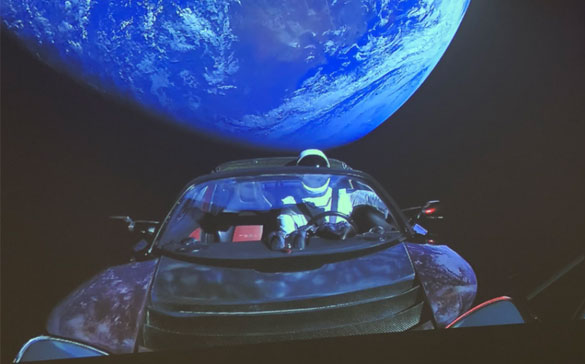
\includegraphics[width=0.5\textwidth]{tesla.jpg}
%\caption{\label{fig:tesla}Esta imagen se añadió en el menú Project.}
%\end{figure}


\subsection{The Newmark's method without damping}


If we start at the beginning, the equation for the elastodynamics model means

\begin{align}
\rho \frac{\partial^2 u}{\partial t^2} & = E  \frac{\partial^2 u}{\partial x^2} \text{ in } (0,L) \times (0,T) \label{e1}\\
u(0,t) & = u^0(t) \text{ in } (0,T) \label{e2}\\
u(L,t) & = u^{N_x}(t)  \text{ in } (0,T) \label{e3} \\
u(x,0) & = u_0(x)  \text{ in } (0,L) \label{e4}\\
\dot{u}(x,0) &  = v_0(x)  \text{ in } (0,T) \label{e5}
\end{align}
Take $i\Delta x = i L/N_x = x_i$ and $u^{i}(t):=u(x_i,t)$  for $0 \le i \le N_x.$ Then \eqref{e1} means
\begin{align}
\frac{\rho}{E} \frac{\partial^2 u^i}{\partial t^2}  = \frac{1}{2\Delta x^2} \left(u^{i+1}(t) -2u^i(t)+u^{i-1}(t)\right),
\end{align}
that is
\begin{align}
\frac{\rho}{E} \ddot{u}^i(t)  = \frac{1}{2\Delta x^2} \left(u^{i+1}(t) -2u^i(t)+u^{i-1}(t)\right), \label{1eq1}
\end{align}
for $1 \le i \le N_x-1.$ Take
$$
\mathbf{u}(t):=(u^1(t),\ldots,u^{N_x-1}(t))^T \in \mathbb{R}^{N_x-1}
$$
and write \eqref{1eq1} as
\begin{align}
M \ddot{\mathbf{u}}(t)  + K \mathbf{u}(t) = \mathbf{F}(t) \label{Peq}
\end{align}
where $M = \frac{\rho}{E} \, id_{(N_x-1) \times (N_x-1)},$ 
$$
K = \left[
\begin{array}{ccccccc}
-2 & 1 & 0 & \cdots & 0 & 0 & 0 \\
1 & -2 & 1 & \cdots & 0 & 0 & 0 \\
0 & 1 & -2 & \cdots & 0 & 0 & 0 \\
\vdots & \vdots & \vdots & \ddots & \vdots & \vdots & \vdots \\
0 & 0 & 0 & \cdots & 1 & -2 & 1 \\
0 & 0 & 0 & \cdots & 0 & 1 & -2
\end{array}
\right]_{(N_x-1) \times (N_x-1)}
$$
is the matrix of discrete Laplacian and, finally,
$$
\mathbf{F}(t) = -\frac{1}{2\Delta x^2}\,(u^0(t),0,\ldots,0,u^{N_x}(t))^T.
$$
Now, consider $t_i = i \,\Delta t = i \, T/N_t$ and 
$$
\mathbf{u}(t_i) = (u^1(t_i),\ldots,u^{N_x-1}(t_i))^T = (u^1_i,\ldots,u^{N_x-1}_i) \in \mathbb{R}^{N_x-1}
$$
for $0 \le i \le N_t.$ We known
$$
\mathbf{u}(t_0) = (u(x_1,0),\ldots,u(x_{N_x-1},0))^T = (u_0(x_1),\ldots,u_0(x_{N_x-1}))^T.
$$
%%%%%%%  PAGINA 1

and

$$
\dot{\mathbf{u}}(t_0) = (\dot{u}(x_1,0),\ldots,\dot{u}(x_{N_x-1},0))^T = (v_0(x_1),\ldots,v_0(x_{N_x-1}))^T.
$$

%%%%% Newmark
Then the Newmark's method reads (see for example \cite{LP2019} p.265--270)
\begin{align}
\dot{\mathbf{u}}(t_i) &z = \dot{\mathbf{u}}(t_{i-1}) + \Delta t (1-\gamma) \ddot{\mathbf{u}}(t_{i-1}) + \Delta t \gamma  \ddot{\mathbf{u}}(t_{i}) \label{N1}\\
\mathbf{u}(t_i) & = \mathbf{u}(t_{i-1})+\Delta t  \dot{\mathbf{u}(t_{i-1})}
+(1-2\beta)\frac{\Delta t^2}{2} \ddot{\mathbf{u}(t_{i-1})}+\beta \Delta t^2  \ddot{\mathbf{u}(t_{i})} \label{N2}
\end{align}
Rearranging \eqref{N2} to provide an expression for $ \ddot{\mathbf{u}}(t_{i})$ that dividing by $\beta \Delta t^2$ gives us
\begin{align}
\ddot{\mathbf{u}}(t_{i}) = \frac{\mathbf{u}(t_{i})-\mathbf{u}(t_{i-1})}{\beta \Delta t^2} - \frac{1}{\beta \Delta t} \dot{\mathbf{u}}(t_{i-1})
-\left( \frac{1}{2\beta}-1\right)\ddot{\mathbf{u}}(t_{i-1}), \label{ddot1}
\end{align}
and, inserting the expression for $\ddot{\mathbf{u}}(t_{i})$ from above into \eqref{N1} gives:
\begin{align}
\dot{\mathbf{u}}(t_{i}) = \frac{\gamma(\mathbf{u}(t_{i})-\mathbf{u}(t_{i-1}))}{\beta \Delta t} + \left( 1 - \frac{\gamma}{\beta }\right)  \dot{\mathbf{u}}(t_{i-1})
+\Delta t \left( 1-\frac{\gamma}{2\beta}\right)\ddot{\mathbf{u}}(t_{i-1}) \label{dot1}
\end{align}
We insert the explicit expression of \eqref{N2} into \eqref{Peq} to obtain
\begin{align}
 M \ddot{\mathbf{u}}(t_{i})  + K \left(\mathbf{u}(t_{i-1}) + \Delta t \dot{\mathbf{u}}(t_{i-1})
- \Delta t^2 \left( \beta -\frac{1}{2}\right)\ddot{\mathbf{u}}(t_{i-1}) + \Delta t^2 \beta \ddot{\mathbf{u}}(t_{i}) \right)   = \mathbf{F}(t_{i})\label{newmark}
\end{align}
and where
$$
\ddot{\mathbf{u}}(t_0) = M^{-1}\left( \mathbf{F}(t_0) - K \mathbf{u}(t_0) \right).
$$
Now, put
\begin{align*}
\mathbf{U} & = \left[\mathbf{u}(t_1) \mathbf{u}(t_2) \cdots \mathbf{u}(t_{N_t})\right] \in \mathbb{R}^{(N_x-1) \times N_t} \\
\dot{\mathbf{U}} & = \left[\dot{\mathbf{u}}(t_1) \dot{\mathbf{u}}(t_2) \cdots \dot{\mathbf{u}}(t_{N_t})\right] \in \mathbb{R}^{(N_x-1) \times N_t} \\
\ddot{\mathbf{U}} & = \left[\ddot{\mathbf{u}}(t_1) \ddot{\mathbf{u}}(t_2) \cdots \ddot{\mathbf{u}}(t_{N_t})\right] \in \mathbb{R}^{(N_x-1) \times N_t} 
\end{align*}
and define
$$
\mathrm{vec}(\mathbf{U}) = \left[
\begin{array}{c}
\mathbf{u}(t_1)\\
\mathbf{u}(t_2) \\
\vdots \\
\mathbf{u}(t_{N_t}) 
\end{array}
\right] \in \mathbb{R}^{N_t(N_x-1)}.
$$
Then we can write \eqref{newmark}  as
\begin{align*}
\left[
\begin{array}{ccccccc}
\Delta t^2 \beta K + M & 0 & 0  &\cdots & 0 & 0 & 0 \\
\Delta t^2 \left( \frac{1}{2} - \beta \right) K & \Delta t^2 \beta K + M & 0 & \cdots & 0 & 0 & 0 \\
0 & \Delta t^2 \left( \frac{1}{2} - \beta \right) K & \Delta t^2 \beta K + M & \cdots & 0 & 0 & 0 \\
\vdots & \vdots & \vdots & \ddots & \vdots & \vdots & \vdots \\
0 & 0 & 0 & \cdots & \Delta t^2 \left( \frac{1}{2} - \beta \right) K & \Delta t^2 \beta K + M & 0 \\
0 & 0 & 0 & \cdots & 0 & \Delta t^2 \left( \frac{1}{2} - \beta \right) K  & \Delta t^2 \beta K + M \\
\end{array}
\right]\left[
\begin{array}{c}
\ddot{\mathbf{u}}(t_1)\\
\ddot{\mathbf{u}}(t_2) \\
\vdots \\
\ddot{\mathbf{u}}(t_{N_t}) 
\end{array}
\right] +  \\
\Delta t \left[
\begin{array}{ccccccc}
0 & 0 & 0  &\cdots & 0 & 0 & 0 \\
 K & 0 & 0 & \cdots & 0 & 0 & 0 \\
0 & K & 0 & \cdots & 0 & 0 & 0 \\
\vdots & \vdots & \vdots & \ddots & \vdots & \vdots & \vdots \\
0 & 0 & 0 & \cdots & K & 0 & 0 \\
0 & 0 & 0 & \cdots & 0 & K  & 0 \\
\end{array}
\right]\left[
\begin{array}{c}
\dot{\mathbf{u}}(t_1)\\
\dot{\mathbf{u}}(t_2) \\
\vdots \\
\dot{\mathbf{u}}(t_{N_t}) 
\end{array}
\right] + \\
\left[
\begin{array}{ccccccc}
0 & 0 & 0  &\cdots & 0 & 0 & 0 \\
 K & 0 & 0 & \cdots & 0 & 0 & 0 \\
0 & K & 0 & \cdots & 0 & 0 & 0 \\
\vdots & \vdots & \vdots & \ddots & \vdots & \vdots & \vdots \\
0 & 0 & 0 & \cdots & K & 0 & 0 \\
0 & 0 & 0 & \cdots & 0 & K  & 0 \\
\end{array}
\right]\left[
\begin{array}{c}
\mathbf{u}(t_1)\\
\mathbf{u}(t_2) \\
\vdots \\
\mathbf{u}(t_{N_t}) 
\end{array}
\right] =
\left[
\begin{array}{c}
\mathbf{F}(t_1)\\
\mathbf{F}(t_2) \\
\vdots \\
\mathbf{F}(t_{N_t}) 
\end{array}
\right] + 
\left[
\begin{array}{c}
-  K  \mathbf{u}(t_0) - \Delta t K \dot{\mathbf{u}}(t_0) - \Delta t^2 \left( \frac{1}{2}-\beta \right) K \ddot{\mathbf{u}}(t_0)\\
\mathbf{0} \\
\vdots \\
\mathbf{0} 
\end{array}
\right],
\end{align*}

%%%%%%%%%% PAGINA 2


that is
\begin{align}
\begin{array}{c}
\left(D_0 \otimes K + id_{N_t \times N_t} \otimes  M  \right) \mathrm{vec}(\ddot{\mathbf{U}}) - \Delta t \left(D_4 \otimes  \frac{M}{\beta\, \Delta t^2}\right)\mathrm{vec}(\dot{\mathbf{U}}) \\
- \left( D_4 \otimes   K\right)\mathrm{vec}(\mathbf{U}) =
\mathbf{a},
\end{array}\label{newmark1}
\end{align}
where
$$
D_0 := \left[
\begin{array}{cccccc}
\Delta t^2 \beta  & 0 & 0 & \cdots & 0 & 0 \\
\Delta t^2 \left(\frac{1}{2} - \beta \right) & \Delta t^2 \beta & 0 & \cdots & 0 & 0 \\
0 & \Delta t^2 \left(\frac{1}{2} - \beta \right) & \Delta t^2 \beta & \cdots & 0 & 0 \\
\vdots & \vdots & \vdots & \ddots & \vdots & \vdots \\
0 & 0 & 0 & \cdots & \Delta t^2 \beta & 0 \\
0 & 0 & 0 & \cdots & \Delta t^2 \left(\frac{1}{2} - \beta \right) & \Delta t^2 \beta  
\end{array}  
\right],
$$
$$
D_4 := \left[
\begin{array}{cccccc}
0  & 0 & 0 & \cdots & 0 & 0 \\
-1 & 0 & 0 & \cdots & 0 & 0 \\
0 & -1 & 0 & \cdots & 0 & 0 \\
\vdots & \vdots & \vdots & \ddots & \vdots & \vdots \\
0 & 0 & 0 & \cdots & 0 & 0 \\
0 & 0 & 0 & \cdots & -1 & 0 
\end{array}  
\right],
$$
$$
\mathbf{a}:= \left[
\begin{array}{c}
\mathbf{F}(t_1)\\
\mathbf{F}(t_2) \\
\vdots \\
\mathbf{F}(t_{N_t}) 
\end{array}
\right] + 
\left[
\begin{array}{c}
-  K  \mathbf{u}(t_0) - \Delta t K \dot{\mathbf{u}}(t_0) - \Delta t^2 \left( \frac{1}{2}-\beta \right) K \ddot{\mathbf{u}}(t_0)\\
\mathbf{0} \\
\vdots \\
\mathbf{0} 
\end{array}
\right].
$$


Proceeding in a similar way with \eqref{N1} and \eqref{N2} we obtain
\begin{align*}
\left[
\begin{array}{ccccccc}
id_{(N_x-1)\times(N_x-1)}& 0 & 0  &\cdots & 0 & 0 \\
 -id_{(N_x-1)\times(N_x-1)} & id_{(N_x-1)\times(N_x-1)} & 0 & \cdots & 0 & 0 \\
0 & -id_{(N_x-1)\times(N_x-1)} & id_{(N_x-1)\times(N_x-1)} & \cdots & 0 & 0 \\
\vdots & \vdots & \vdots & \ddots & \vdots & \vdots \\
0 & 0 & 0 & \cdots & id_{(N_x-1)\times(N_x-1)}  & 0 \\
0 & 0 & 0 & \cdots & -id_{(N_x-1)\times(N_x-1)} &  id_{(N_x-1)\times(N_x-1)} \\
\end{array}
\right]\left[
\begin{array}{c}
\dot{\mathbf{u}}(t_1)\\
\dot{\mathbf{u}}(t_2) \\
\vdots \\
\dot{\mathbf{u}}(t_{N_t}) 
\end{array}
\right] -
\end{align*}
\begin{align*}
\Delta t\left[
\begin{array}{cccccc}
 \gamma id_{(N_x-1)\times(N_x-1)} & 0 & 0  &\cdots & 0 & 0 \\
 \left(1-\gamma\right)id_{(N_x-1)\times(N_x-1)} & \gamma id_{(N_x-1)\times(N_x-1)} & 0 &  \cdots & 0 & 0  \\
\vdots & \vdots & \vdots & \ddots & \vdots & \vdots  \\
0 & 0 & 0 &\cdots & \left(1-\gamma\right)id_{(N_x-1)\times(N_x-1)} & \gamma id_{(N_x-1)\times(N_x-1)}
\end{array}
\right]\left[
\begin{array}{c}
\ddot{\mathbf{u}}(t_1)\\
\ddot{\mathbf{u}}(t_2) \\
\vdots \\
\ddot{\mathbf{u}}(t_{N_t}) 
\end{array}
\right] = \\
\left[
\begin{array}{c}
\dot{\mathbf{u}}(t_0) + \left(1-\gamma\right)\Delta t\ddot{\mathbf{u}}(t_0) \\
\mathbf{0} \\
\vdots \\
\mathbf{0} 
\end{array}
\right],
\end{align*}


%%%%%%%%%% PAGINA 3



Introduce the following two matrices
$$
D_1 = \left[
\begin{array}{cccccc}
1 & 0 & 0 & \cdots & 0 & 0 \\
-1 & 1 & 0 & \cdots & 0 & 0 \\
0 & -1 & 1 & \cdots & 0 & 0 \\
\vdots & \vdots & \vdots & \ddots & \vdots & \vdots \\
0 & 0 & 0 & \cdots & 1 & 0 \\
0 & 0 & 0 & \cdots & -1 & 1  
\end{array}  
\right]
\text{ and } 
D_2 = \left[
\begin{array}{cccccc}
\gamma & 0 & 0 & \cdots & 0 & 0 \\
\left( 1-\gamma \right) & \gamma & 0 & \cdots & 0 & 0 \\
0 & \left( 1-\gamma\right) & 1 & \cdots & 0 & 0 \\
\vdots & \vdots & \vdots & \ddots & \vdots & \vdots \\
0 & 0 & 0 & \cdots & \gamma & 0 \\
0 & 0 & 0 & \cdots & \left(1-\gamma\right) & \gamma 
\end{array}  
\right].
$$
Observe that 
$$
D_1^{-1} = \left[
\begin{array}{cccccc}
1 & 0 & 0 & \cdots & 0 & 0 \\
1 & 1 & 0 & \cdots & 0 & 0 \\
1 & 1 & 1 & \cdots & 0 & 0 \\
\vdots & \vdots & \vdots & \ddots & \vdots & \vdots \\
1 & 1 & 1 & \cdots & 1 & 0 \\
1 & 1 & 1 & \cdots & 1 & 1  
\end{array}  
\right].
$$
Then \eqref{ddot1} can be written as
\begin{align}
\begin{array}{c}
\left( D_1 \otimes  id_{(N_x-1)\times(N_x-1)}\right) \mathrm{vec}(\dot{\mathbf{U}}) - \Delta t \left( D_2 \otimes  id_{(N_x-1)\times(N_x-1)}\right) \mathrm{vec}(\ddot{\mathbf{U}}) = \mathbf{b}
\end{array}\label{newmark2}
\end{align}
where
$$
\mathbf{b}:= \left[
\begin{array}{c}
\dot{\mathbf{u}}(t_0) + \left(1-\gamma\right)\Delta t\ddot{\mathbf{u}}(t_0) \\
\mathbf{0} \\
\vdots \\
\mathbf{0} 
\end{array}
\right].
$$
Thus,
$$
\mathrm{vec}(\dot{\mathbf{U}}) = \left( D_1^{-1} \otimes  id_{(N_x-1)\times(N_x-1)}\right)\left( \mathbf{b} +  \Delta t \left( D_2 \otimes  id_{(N_x-1)\times(N_x-1)}\right) \mathrm{vec}(\ddot{\mathbf{U}})\right)
$$

Finally, we can compute \eqref{N2} following the same strategy to obtain by using the matrix
$$
D_3 = \left[
\begin{array}{cccccc}
\beta & 0 & 0 & \cdots & 0 & 0 \\
\frac{1}{2}-\beta  & \beta & 0 & \cdots & 0 & 0 \\
0 &\frac{1}{2}-\beta  & \beta & \cdots & 0 & 0 \\
\vdots & \vdots & \vdots & \ddots & \vdots & \vdots \\
0 & 0 & 0 & \cdots & \beta & 0 \\
0 & 0 & 0 & \cdots &\frac{1}{2}-\beta & \beta 
\end{array}  
\right].
$$
We obtain
\begin{align}
\begin{array}{c}
\left( D_1 \otimes  id_{(N_x-1)\times(N_x-1)}\right) \mathrm{vec}(\mathbf{U}) + \Delta t
\left(D_4 \otimes  id_{(N_x-1)\times(N_x-1)} \right)\mathrm{vec}(\dot{\mathbf{U}}) \\ - \Delta t^2 \left( D_3 \otimes  id_{(N_x-1)\times(N_x-1)} \right) \mathrm{vec}(\ddot{\mathbf{U}}) = \mathbf{c}
\end{array}\label{newmark3}
\end{align}\
where
$$
\mathbf{c}:= \left[
\begin{array}{c}
\mathbf{u}(t_0) + \Delta t \, \dot{\mathbf{u}}(t_0) + \Delta t^2 \left(\frac{1}{2}-\beta\right)\ddot{\mathbf{u}}(t_0)+  \\
\mathbf{0} \\
\vdots \\
\mathbf{0} 
\end{array}
\right].
$$

\bigskip

%%%%%%%%% PAGINA 4



We remark that
\begin{align*}
\mathrm{vec}(\mathbf{U}) =\left( D_1^{-1} \otimes  id_{(N_x-1)\times(N_x-1)}\right) \times \\
\left( \mathbf{c} - 
\Delta t
\left(D_4 \otimes  id_{(N_x-1)\times(N_x-1)} \right)\mathrm{vec}(\dot{\mathbf{U}}) + \Delta t^2 \left( D_3 \otimes  id_{(N_x-1)\times(N_x-1)} \right) \mathrm{vec}(\ddot{\mathbf{U}})
\right) 
\end{align*}
where
$$
\mathrm{vec}(\dot{\mathbf{U}}) = \left( D_1^{-1} \otimes  id_{(N_x-1)\times(N_x-1)}\right)\left( \mathbf{b} +  \Delta t \left( D_2 \otimes  id_{(N_x-1)\times(N_x-1)}\right) \mathrm{vec}(\ddot{\mathbf{U}})\right).
$$
By substituting both in \eqref{newmark1} we obtain:
$$
\begin{array}{c}
\left(D_0 \otimes K + id_{N_t \times N_t} \otimes  M  \right) \mathrm{vec}(\ddot{\mathbf{U}}) - \Delta t \left(D_4 \otimes  K \right) \\
\times \left( D_1^{-1} \otimes  id_{(N_x-1)\times(N_x-1)}\right) \times \left( \mathbf{b} +  \Delta t \left( D_2 \otimes  id_{(N_x-1)\times(N_x-1)}\right) \mathrm{vec}(\ddot{\mathbf{U}})\right) \\ 
 -  \left( D_4 \otimes   K\right) \times \left( D_1^{-1} \otimes  id_{(N_x-1)\times(N_x-1)}\right) \\ 
\times \left( \mathbf{c} - \Delta t \left(D_4 \otimes  id_{(N_x-1)\times(N_x-1)} \right) \times \left( D_1^{-1} \otimes  id_{(N_x-1)\times(N_x-1)}\right) \right. \\
\left. \times \left( \mathbf{b} +  \Delta t \left( D_2 \otimes  id_{(N_x-1)\times(N_x-1)}\right) \mathrm{vec}(\ddot{\mathbf{U}})\right) + \Delta t^2 \left( D_3 \otimes  id_{(N_x-1)\times(N_x-1)} \right) \mathrm{vec}(\ddot{\mathbf{U}}) \right)   =
\mathbf{a},
\end{array}
$$

that is a linear equation in $\mathrm{vec}(\ddot{\mathbf{U}}).$ So we can get $\mathrm{vec}(\ddot{\mathbf{U}})$ as follows:

$$
\begin{array}{c}
\mathrm{vec}(\ddot{\mathbf{U}}) = \left(\left(D_0 \otimes K + id_{N_t \times N_t} \otimes  M  \right) - \Delta t \left(D_4 \otimes  K \right) \times \left( D_1^{-1} \otimes  id_{(N_x-1)\times(N_x-1)}\right)   \right.\\
\left. \Delta t \left( D_2 \otimes  id_{(N_x-1)\times(N_x-1)}\right) -  \left( D_4 \otimes   K\right) \times \left( D_1^{-1} \otimes  id_{(N_x-1)\times(N_x-1)}\right) \right. \\
\left.  \times \left( - \Delta t \left(D_4 \otimes  id_{(N_x-1)\times(N_x-1)} \right) \times \left( D_1^{-1} \otimes  id_{(N_x-1)\times(N_x-1)}\right) \right. \right. \\
\left. \left. \Delta t \left( D_2 \otimes  id_{(N_x-1)\times(N_x-1)}\right)  + \Delta t^2 \left( D_3 \otimes  id_{(N_x-1)\times(N_x-1)} \right) \right) \right)^{-1} \\
\times \left( \Delta t \left(D_4 \otimes  K \right) \times \left( D_1^{-1} \otimes  id_{(N_x-1)\times(N_x-1)}\right)  \mathbf{b} +\left( D_4 \otimes   K\right) \times \left( D_1^{-1} \otimes  id_{(N_x-1)\times(N_x-1)}\right) \right. \\
\left.  \times \left( - \Delta t \left(D_4 \otimes  id_{(N_x-1)\times(N_x-1)} \right) \times \left( D_1^{-1} \otimes  id_{(N_x-1)\times(N_x-1)}\right) \mathbf{b}  + \mathbf{c}  \right) + \mathbf{a}  \right), \\
\end{array}
$$





\subsection{The Newmark's method with damping}


As has been done in the previous section, we can write \eqref{1eq1} including damping as follows
\begin{align}
M \ddot{\mathbf{u}}(t) + C \dot{\mathbf{u}}(t)  + K \mathbf{u}(t) = \mathbf{F}(t) \label{PeqC}
\end{align}
We insert the explicit expression of \eqref{N2} into \eqref{PeqC} to obtain
\begin{align}
 M \ddot{\mathbf{u}}(t_{i})  + C \left(\dot{\mathbf{u}}(t_{i-1})
- \Delta t \left( \gamma -1\right)\ddot{\mathbf{u}}(t_{i-1}) + \Delta t \gamma \ddot{\mathbf{u}}(t_{i}) \right) \\
+ K \left(\mathbf{u}(t_{i-1}) + \Delta t \dot{\mathbf{u}}(t_{i-1})
- \Delta t^2 \left( \beta -\frac{1}{2}\right)\ddot{\mathbf{u}}(t_{i-1}) + \Delta t^2 \beta \ddot{\mathbf{u}}(t_{i}) \right)   = \mathbf{F}(t_{i})\label{newmarkC}
\end{align}
and where
$$
\ddot{\mathbf{u}}(t_0) = M^{-1}\left( \mathbf{F}(t_0) - C \dot{\mathbf{u}}(t_0) - K \mathbf{u}(t_0) \right).
$$
Then we can write \ref{newmarkC} as
\begin{align}
\begin{array}{c}
\left(D_0 \otimes K + \Delta t D_2 \otimes C + id_{N_t \times N_t} \otimes  M  \right) \mathrm{vec}(\ddot{\mathbf{U}}) - \left(D_4 \otimes  \left(C+\Delta t K\right)\right)\mathrm{vec}(\dot{\mathbf{U}}) \\
- \left( D_4 \otimes   K\right)\mathrm{vec}(\mathbf{U}) =
\mathbf{a},
\end{array}\label{newmark1}
\end{align}
There is only a vector that changes from previous section being now
$$
\mathbf{a}:= \left[
\begin{array}{c}
\mathbf{F}(t_1)\\
\mathbf{F}(t_2) \\
\vdots \\
\mathbf{F}(t_{N_t}) 
\end{array}
\right] + 
\left[
\begin{array}{c}
-  K  \mathbf{u}(t_0) - \left( C + \Delta t K \right) \dot{\mathbf{u}}(t_0) - \left( \Delta t \left(1 - \gamma \right) C + \Delta t^2 \left( \frac{1}{2}-\beta \right) K \right)\ddot{\mathbf{u}}(t_0)\\
\mathbf{0} \\
\vdots \\
\mathbf{0} 
\end{array}
\right].
$$
Proceeding in the same way as past section we can get $\mathrm{vec}(\ddot{\mathbf{U}})$ as follows:
$$
\begin{array}{c}
\mathrm{vec}(\ddot{\mathbf{U}}) = \left(\left(D_0 \otimes K + \Delta t D_2 \otimes C + id_{N_t \times N_t} \otimes  M  \right) - \left(D_4 \otimes  \left(C+\Delta t K\right)\right) \times \left( D_1^{-1} \otimes  id_{(N_x-1)\times(N_x-1)}\right)   \right.\\
\left. \Delta t \left( D_2 \otimes  id_{(N_x-1)\times(N_x-1)}\right) -  \left( D_4 \otimes   K \right) \times \left( D_1^{-1} \otimes  id_{(N_x-1)\times(N_x-1)}\right) \right. \\
\left.  \times \left( - \Delta t \left(D_4 \otimes  id_{(N_x-1)\times(N_x-1)} \right) \times \left( D_1^{-1} \otimes  id_{(N_x-1)\times(N_x-1)}\right) \right. \right. \\
\left. \left. \Delta t \left( D_2 \otimes  id_{(N_x-1)\times(N_x-1)}\right)  + \Delta t^2 \left( D_3 \otimes  id_{(N_x-1)\times(N_x-1)} \right) \right) \right)^{-1} \\
\times \left( \left(D_4 \otimes  \left( C + \Delta t K\right) \right) \times \left( D_1^{-1} \otimes  id_{(N_x-1)\times(N_x-1)}\right)  \mathbf{b} +\left( D_4 \otimes   K\right) \times \left( D_1^{-1} \otimes  id_{(N_x-1)\times(N_x-1)}\right) \right. \\
\left.  \times \left( - \Delta t \left(D_4 \otimes  id_{(N_x-1)\times(N_x-1)} \right) \times \left( D_1^{-1} \otimes  id_{(N_x-1)\times(N_x-1)}\right) \mathbf{b}  + \mathbf{c}  \right) + \mathbf{a}  \right), \\
\end{array}
$$




\subsection{Greedy Rank-One Update Algorithm}

The most important part of the simulator deals with the Greedy Rank-One Update Algorithm (or as it has been called GROUA in previous sections). In this section we will try to explain how this method works, as well as the main equations that form it.\\

The method consists of iteratively evaluating a for loop, which extracts a remainder and the acceleration vector as outputs. If this residual is less than a stipulated error, the acceleration vector is correct. If, on the other hand, this remainder is greater than this error, the for loop is executed again. This is reflected in the figure \ref{Main loop}, which is a block diagram that summarizes the operation of the method. As input to the program, the matrix system obtained in the previous section is given, which had been obtained after developing the Newmark equations in a tensorial form.\\


For the case without damping, the input elements are:

$$
\begin{array}{c}
A = \left(D_0 \otimes K + id_{N_t \times N_t} \otimes  M  \right) - \Delta t \left(D_4 \otimes  K \right) \times \left( D_1^{-1} \otimes  id_{(N_x-1)\times(N_x-1)}\right)  \\
\left. \Delta t \left( D_2 \otimes  id_{(N_x-1)\times(N_x-1)}\right) -  \left( D_4 \otimes   K\right) \times \left( D_1^{-1} \otimes  id_{(N_x-1)\times(N_x-1)}\right) \right. \\
\left.  \times \left( - \Delta t \left(D_4 \otimes  id_{(N_x-1)\times(N_x-1)} \right) \times \left( D_1^{-1} \otimes  id_{(N_x-1)\times(N_x-1)}\right) \right. \right.\\
\left. \Delta t \left( D_2 \otimes  id_{(N_x-1)\times(N_x-1)}\right)  + \Delta t^2 \left( D_3 \otimes  id_{(N_x-1)\times(N_x-1)} \right) \right)
\end{array}
$$

$$
\begin{array}{c}
b = \Delta t \left(D_4 \otimes  K \right) \times \left( D_1^{-1} \otimes  id_{(N_x-1)\times(N_x-1)}\right)  \mathbf{b} +\left( D_4 \otimes   K\right) \times \left( D_1^{-1} \otimes  id_{(N_x-1)\times(N_x-1)}\right) \\
 \times \left( - \Delta t \left(D_4 \otimes  id_{(N_x-1)\times(N_x-1)} \right) \times \left( D_1^{-1} \otimes  id_{(N_x-1)\times(N_x-1)}\right) \mathbf{b}  + \mathbf{c}  \right) + \mathbf{a} \\
\end{array}
$$



While for the case with damping the input elements are:

$$
\begin{array}{c}
A = \left(D_0 \otimes K + \Delta t D_2 \otimes C + id_{N_t \times N_t} \otimes  M  \right) - \left(D_4 \otimes  \left(C+\Delta t K\right)\right) \times \left( D_1^{-1} \otimes  id_{(N_x-1)\times(N_x-1)}\right) \\
\left. \Delta t \left( D_2 \otimes  id_{(N_x-1)\times(N_x-1)}\right) -  \left( D_4 \otimes   K \right) \times \left( D_1^{-1} \otimes  id_{(N_x-1)\times(N_x-1)}\right) \right. \\
\left.  \times \left( - \Delta t \left(D_4 \otimes  id_{(N_x-1)\times(N_x-1)} \right) \times \left( D_1^{-1} \otimes  id_{(N_x-1)\times(N_x-1)}\right) \right. \right. \\
 \left. \Delta t \left( D_2 \otimes  id_{(N_x-1)\times(N_x-1)}\right)  + \Delta t^2 \left( D_3 \otimes  id_{(N_x-1)\times(N_x-1)} \right) \right)  \\
\end{array}
$$

$$
\begin{array}{c}
b = \left(D_4 \otimes  \left( C + \Delta t K\right) \right) \times \left( D_1^{-1} \otimes  id_{(N_x-1)\times(N_x-1)}\right)  \mathbf{b} +\left( D_4 \otimes   K\right) \times \left( D_1^{-1} \otimes  id_{(N_x-1)\times(N_x-1)}\right)  \\
  \times \left( - \Delta t \left(D_4 \otimes  id_{(N_x-1)\times(N_x-1)} \right) \times \left( D_1^{-1} \otimes  id_{(N_x-1)\times(N_x-1)}\right) \mathbf{b}  + \mathbf{c}  \right) + \mathbf{a} \\
\end{array}
$$



\begin{figure}
\centering
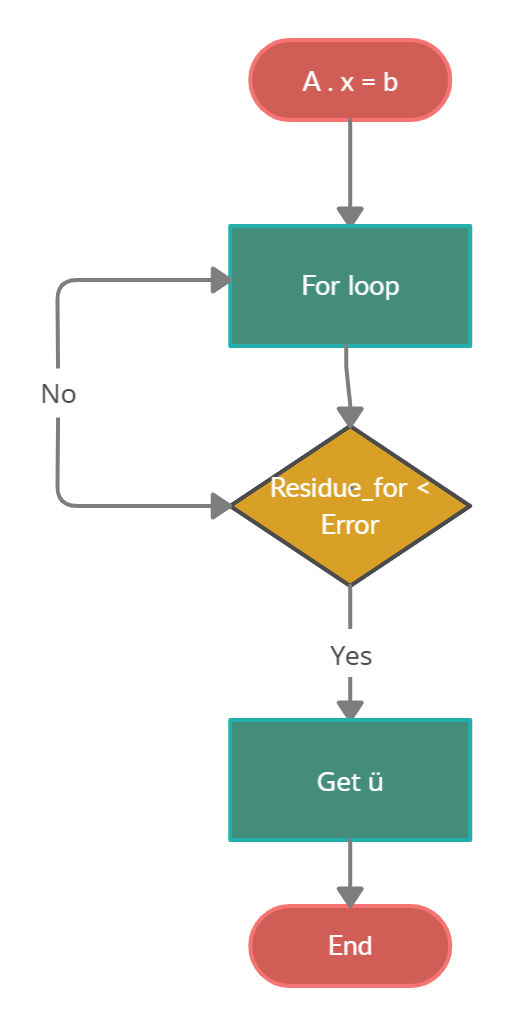
\includegraphics[width=0.30\textwidth]{Main block (1).png}
\caption{Main loop} 
\label{Main loop}
\end{figure}

\newpage

If the for loop itself is analyzed, as can be seen in the figure \ ref {For loop}, its structure is very similar to the structure of the general method. As before, a loop is also iteratively evaluated, in this case called while. As with the main loop, if the extracted residue is less than a tolerance, the necessary outputs are obtained for the evaluation of the upper loop (for loop). If not, the while loop is executed again. Unlike what happened in the other loop, each time the for loop is entered, initial conditions are generated, which are random.


\begin{figure}
\centering
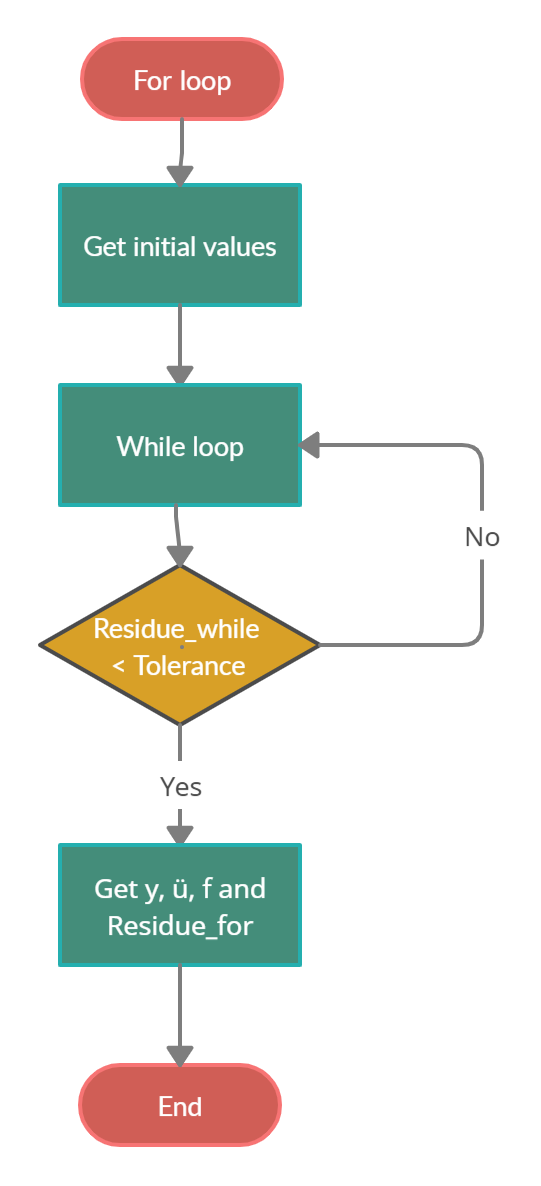
\includegraphics[width=0.30\textwidth]{For loop (1).png}
\caption{For loop} 
\label{For loop}
\end{figure}

The equations found in the while loop and how to proceed are as follows: First the previous value of the vector $x_10$ is saved, which in the first iteration is random.
\begin{equation}
    x_{1} = x_{10}
\end{equation}
After this, the matrix $Z_1$ is generated and the new value of $x_{10}$ is calculated.
\begin{equation}
    Z_1 = A I_t \otimes  x_{20}
\end{equation}
\begin{equation}
    x_{10} = Z_1^{-1} f
\end{equation}
Once the new $x_{10}$ is obtained, the tolerance between this vector and the previously saved one is calculated.
\begin{equation}
    tol_1 = |x_{10}-x_1|
\end{equation}
It proceeds in the same way for all the present state vectors, taking as tolerance the one with the highest absolute value of all of them. The loop will end when said tolerance is less than the one imposed as allowed. After finishing with the while loop, the value of $y$ is updated, being this:
\begin{equation}
    y = x_{10} \otimes  x_{20}
\end{equation}
The accumulation of the different values of $y$ is what will ultimately give the acceleration vector $\ddot{u}$. Although for this it is necessary to carry out several iterations repeating the process, therefore, the variable $fn$ is created, which indicates how close $y$ is to being correct.
\begin{equation}
    fn = f - A y
\end{equation}
From the residue of $fn$, the residue of the for loop itself is obtained in the same way as the previous ones, which must be less than the previously imposed value in order to consider the calculation finished. Until this happens, the value of $fn$ is saved as the next $f$ and starts over.

Once the correct $\ddot{u}$ has been obtained and with what has been explained in the previous points, it is straightforward to obtain $\dot{u}$ and $u$.

%%% Ecuaciones del while




%%%%%%%%%%%%%%%%%%%%%%%%%%%%%%%%%%%%%%%%
%%%%%% SECCIÓN 4 %%%%%%%%%%%%%%%%%%%%%%%
%%%%%%%%%%%%%%%%%%%%%%%%%%%%%%%%%%%%%%%%


\section{About the convergence and stability of the tensor-based Newmark's method}

This section will comment on the stability and convergence studies and their respective results, if any. This study is of utmost importance, mainly because if the method is not stable, it could give inconsistent results or not provide a solution, and if the results are not converged, the results would be erroneous.

%% Estabilidad, referencia de los japos %%

To carry out the study of the stability of the method, it is necessary to differentiate between two cases: for $\frac{1}{2} \gamma \leq \beta$ and for $0 \leq \beta < \frac{1}{2} \ gamma$. Despite having been programmed for both cases, for the study carried out only one of them will be emphasized, since $\beta = \frac{1}{6} < \frac{1}{2} \gamma$.
For this specific case there is a condition that the time step must meet for the method to be stable: $\tau < \sqrt{\frac{1}{(\frac{1}{2} \gamma - \beta) || K^{1/2}||^2}} $.
Therefore, the method is stable as long as the following condition  is fulfilled:
\begin{equation}
    ||\mathbf{u}(t)|| \leq ||\mathbf{u}(0)|| + \sqrt{\frac{C_0}{1-\tau^2 (\frac{1}{2} \gamma - \beta) ||K^{1/2}||^2}t}
\end{equation}
being:
\begin{equation}
    C_0 = ||\dot{\mathbf{u}}(0)||^2 + \tau^2 (\beta - \frac{1}{2} \gamma + \frac{1}{4}) ||K^{1/2} \dot{\mathbf{u}}(0) ||^2 + \tau (K \dot{\mathbf{u}}(0) \cdot \mathbf{u}(0)) + || K^{1/2} \mathbf{u}(0) ||^2 + \tau (\gamma - \frac{1}{2}) || C^{1/2} \dot{\mathbf{u}}(0) ||^2
\end{equation}
For each executed case, the values change, but the condition of the upper equation must always be met to ensure stability. Stability values will be included in the examples to be described later.\\

%% Convergencia, sobre todo convergencia numérica %%

Regarding convergence, knowing that Newmark's method converges adequately, and also that GROUA itself converges numerically, it can be said that the simulator in general converges. This can be seen more clearly in the evolution of the residual as the iterations increase. The figure \ref{ResIter} shows this evolution, making it clear that from iteration 5, the solution has converged. Furthermore, in the same figure the limit that marks the maximum permissible error has been included, allowing the correct convergence of the method to be concluded at a glance. Keep in mind that the value selected for the error is very small, on the order of Y.

In order to better observe the trend, the first residual has been eliminated from the graph, which is very large due to the randomness of the code initially. Furthermore, it has been deemed convenient not to include the value selected for the error ($ 10{-8}$), as happens later.

In order to better observe the trend of the residue, the figure \ref{ResIterLog} has been included, which has the residue on a logarithmic scale. Despite the downward trend, the solution does not improve after iteration 2, although for safety we will say that after iteration 5 the solution has converged. In addition, in this figure the maximum allowed error has been included, in order to make it clear that it is exceeded in the first iterations.

\begin{figure}
\centering
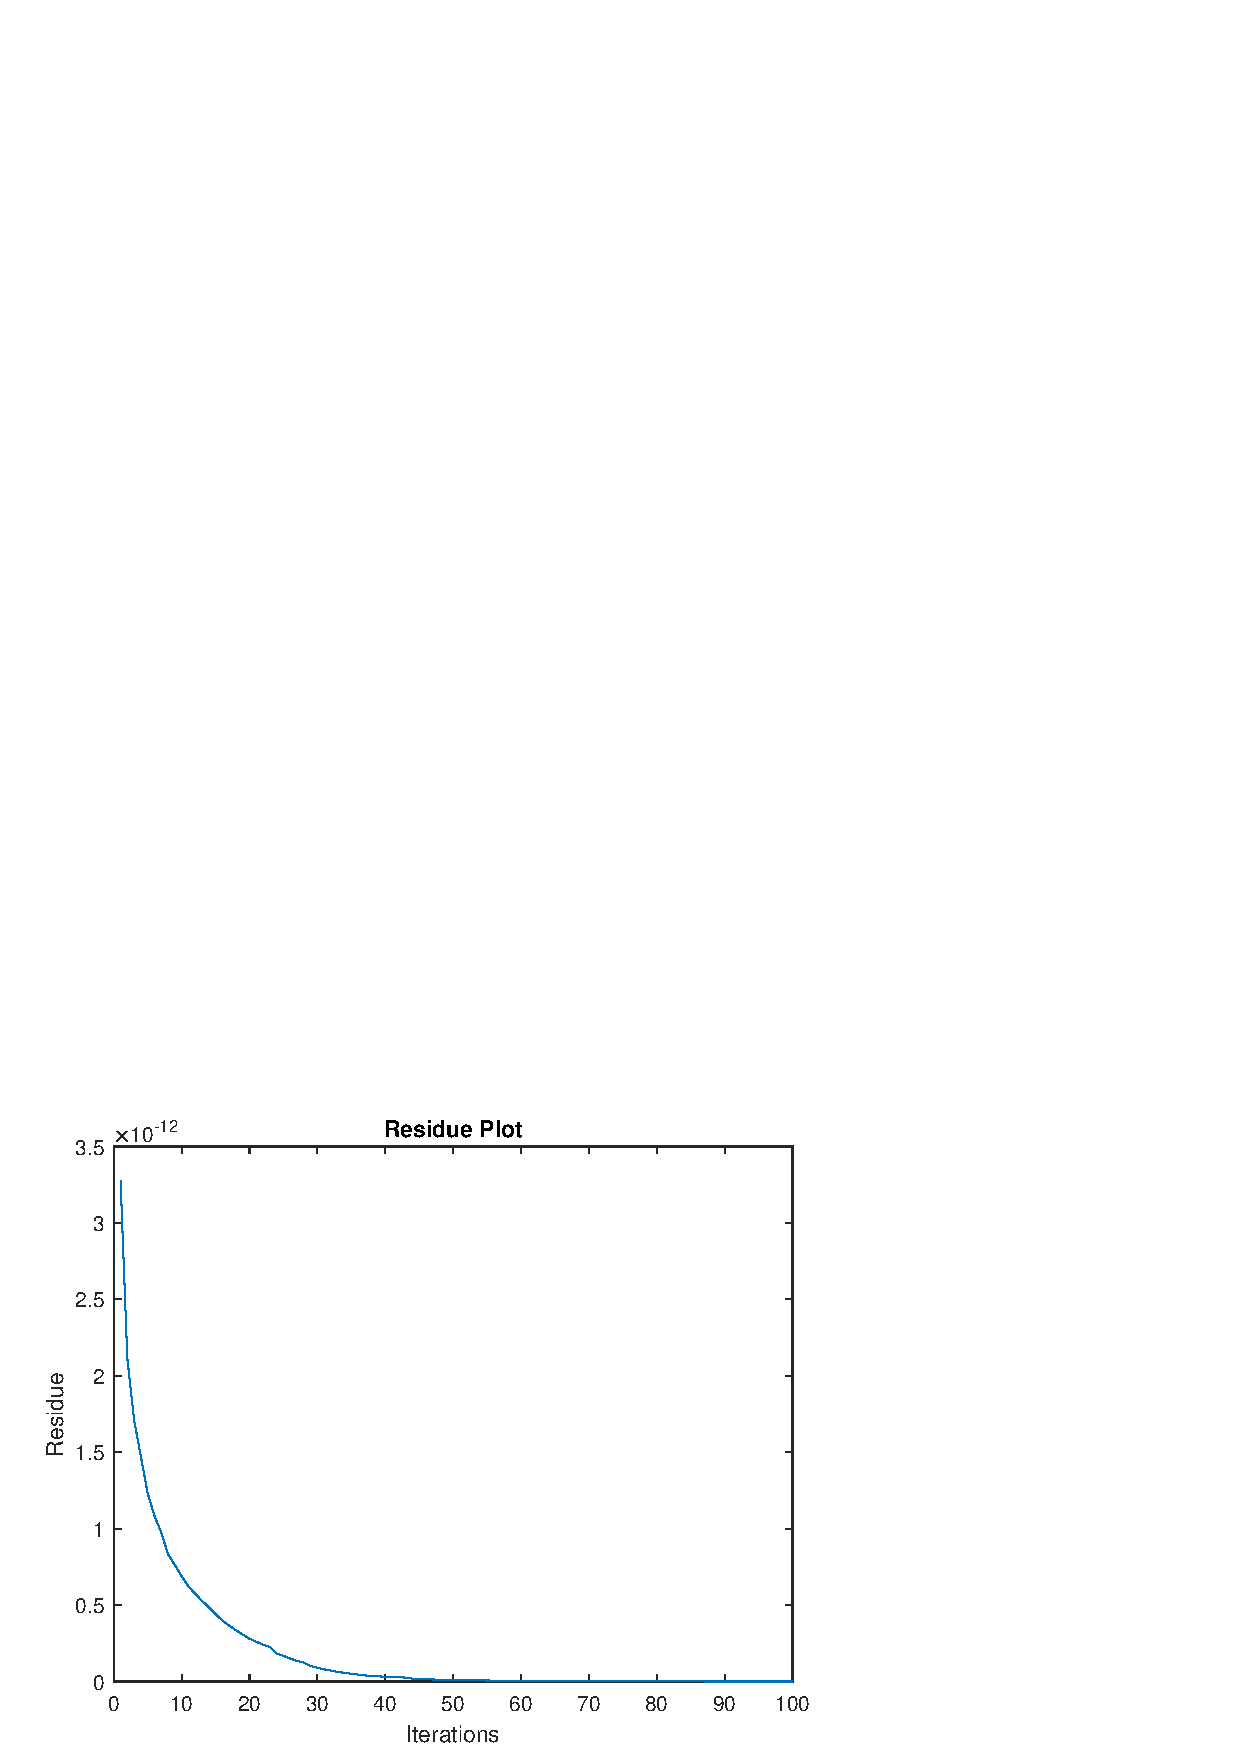
\includegraphics[width=0.75\textwidth]{ResIter}
\caption{Residue evolution vs Iterations } 
\label{ResIter}
\end{figure}

\begin{figure}
\centering
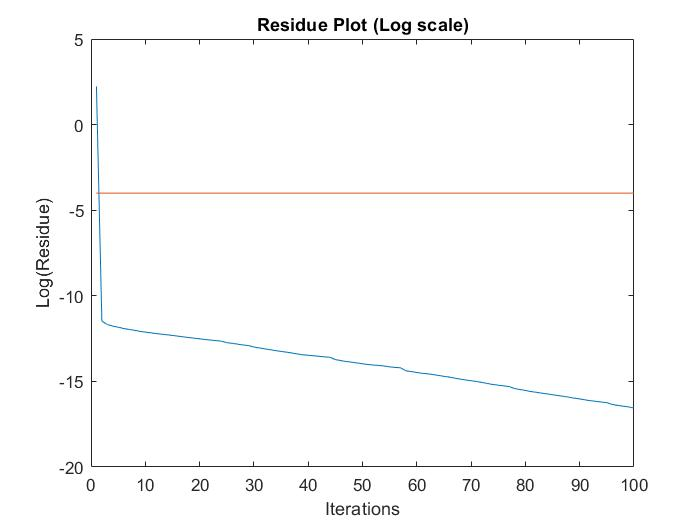
\includegraphics[width=0.75\textwidth]{ResIterLog}
\caption{Residue evolution (Log scale) vs Iterations } 
\label{ResIterLog}
\end{figure}

%%%%%%%%%%%%%%%%%%%%%%%%%%%%%%%%%%%%%%%%
%%%%%% SECCIÓN 5 %%%%%%%%%%%%%%%%%%%%%%%
%%%%%%%%%%%%%%%%%%%%%%%%%%%%%%%%%%%%%%%%

\section{Numerical examples}

In this section everything related to the numerical results obtained will be discussed. Initially, a study that has been carried out on how long the program takes to run will be presented based on the number of spatial and temporal divisions. After this, the numerical examples that have been executed will be shown, both the case without damping and the case with damping.

\subsection{A study of the computational cost of the tensor-based Newmark's method}

In order to better understand how the program works, it has been considered convenient to carry out a small study, to check how the simulator behaves when the temporal and spatial divisions are varied.\\

This study consists of obtaining the simulation times for various cases, and thus being able to analyze their trend. There are three cases studied: variation of spatial divisions, variation of temporal divisions and variation of both.\\


%%%  Space study  %%%

The first study carried out was the one that analyzes the effect of the change in spatial discretization. As can be seen in the figure \ref{SpaceStudy}, the computational cost when using GROUA is always higher. In fact, from 120 divisions, it increases with a greater slope. If you look at the figure \ref{SpaceStudyLog}, you can see how both lines are practically parallel on a logarithmic scale. This allows us to deduce that the cost due to GROUA will never be exceeded by the cost due to the generic resolution.

\begin{figure}
\centering
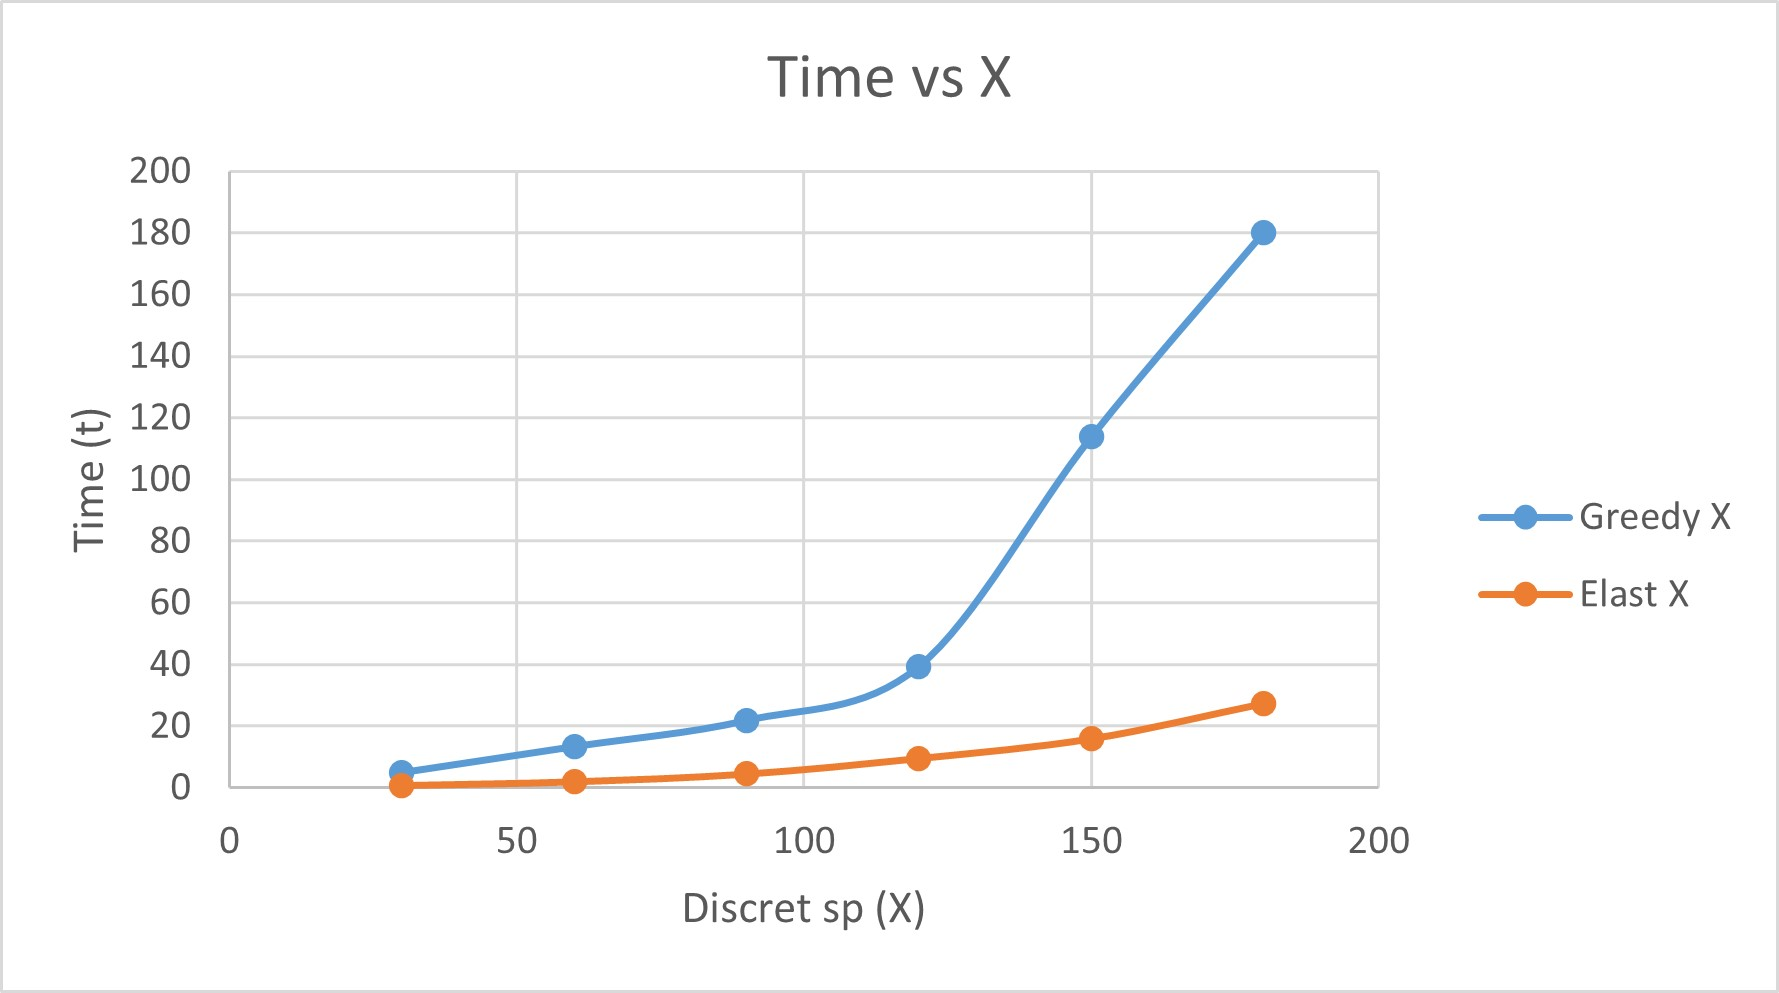
\includegraphics[width=0.75\textwidth]{SpaceStudy.jpg}
\caption{Space study} 
\label{SpaceStudy}
\end{figure}

\begin{figure}
\centering
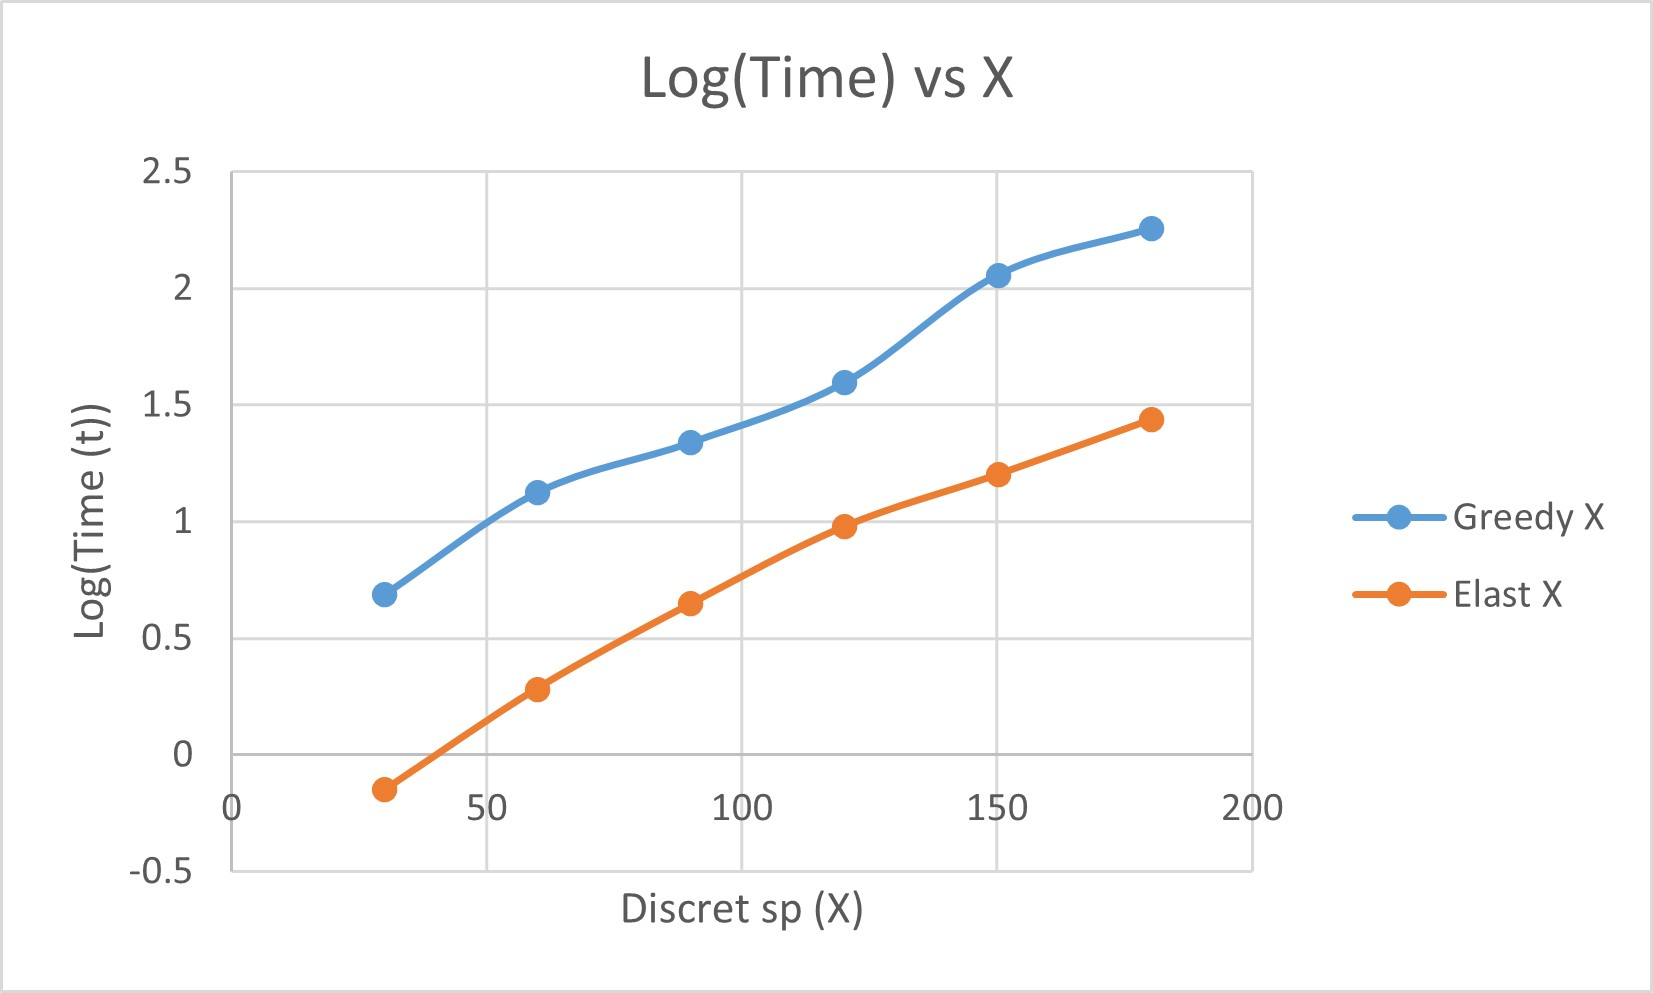
\includegraphics[width=0.75\textwidth]{SpaceStudyLog.jpg}
\caption{Space study (Log scale)} 
\label{SpaceStudyLog}
\end{figure}

%%%  Time study  %%%

Contrary to what happened in the spatial study, for the temporal case there is a certain number of divisions from which the GROUA begins to have a lower cost. As can be seen in the figures \ref{TimeStudy} and \ref{TimeStudyLog}, after 120 divisions the curves intersect, and furthermore, the growth of the generic resolution increases significantly. It could be said that the computational cost of GROUA increases practically linear, while the other increases exponentially.

\begin{figure}
\centering
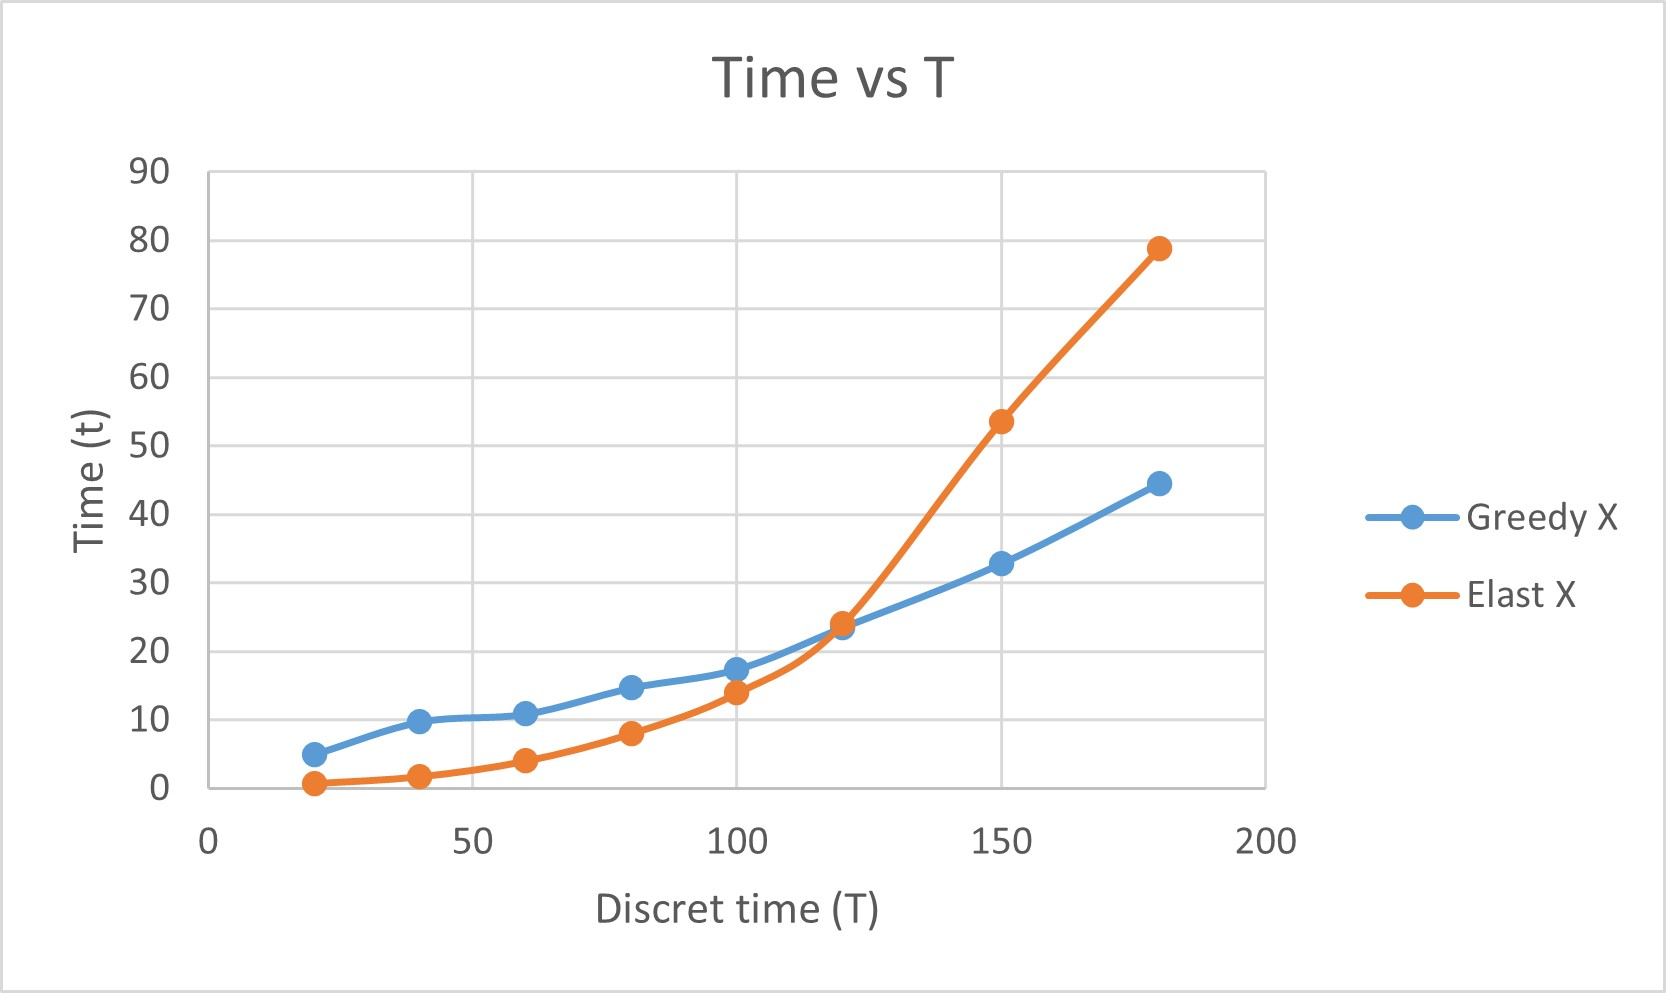
\includegraphics[width=0.75\textwidth]{TimeStudy.jpg}
\caption{Time study} 
\label{TimeStudy}
\end{figure}

\begin{figure}
\centering
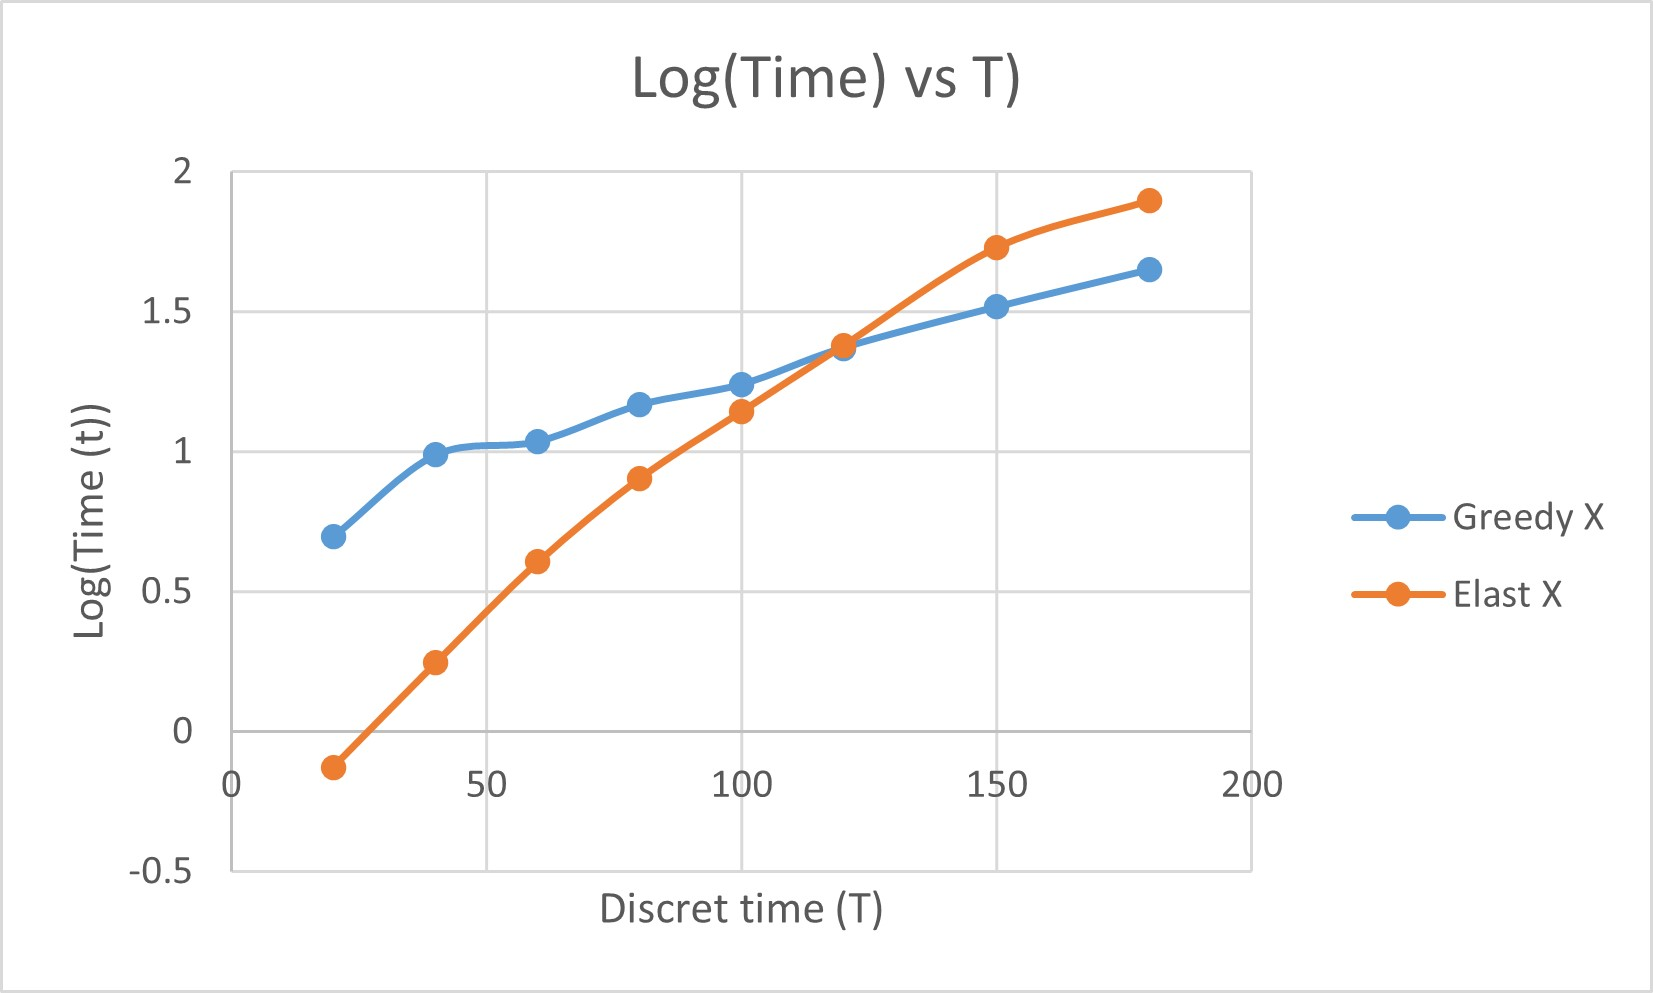
\includegraphics[width=0.75\textwidth]{TimeStudyLog.jpg}
\caption{Time study (Log scale)} 
\label{TimeStudyLog}
\end{figure}

%%%%  Both study  %%%%

After the disparity of the previous results, it was extremely important to analyze the results by changing both discretizations, to see what the trend is in a more real case. As can be seen in the figures \ref{BothStudy} and \ref{BothStudyLog}, there is again a certain number of divisions from which the GROUA has a lower cost. The fundamental differences with respect to the temporal case are that the trend for both cases is exponential and that the number of divisions where they intersect is around 75. It is important to note that the selection of the number of divisions for each case can significantly influence this phenomenon. , although the trend is very similar. Furthermore, it has been decided to represent the solution for this case with respect to the number of temporal divisions, since the only thing that changes is the abscissa axis, but the results for both discretizations are the same.

If the image \ref{BothStudy} is analyzed in greater depth, it can be seen that for the last case the GROUA takes half the time. Furthermore, it is evident that the GROUA curve grows much slower, which will mean that the more divisions the problem has, the greater the differences between the two models.

\begin{figure}
\centering
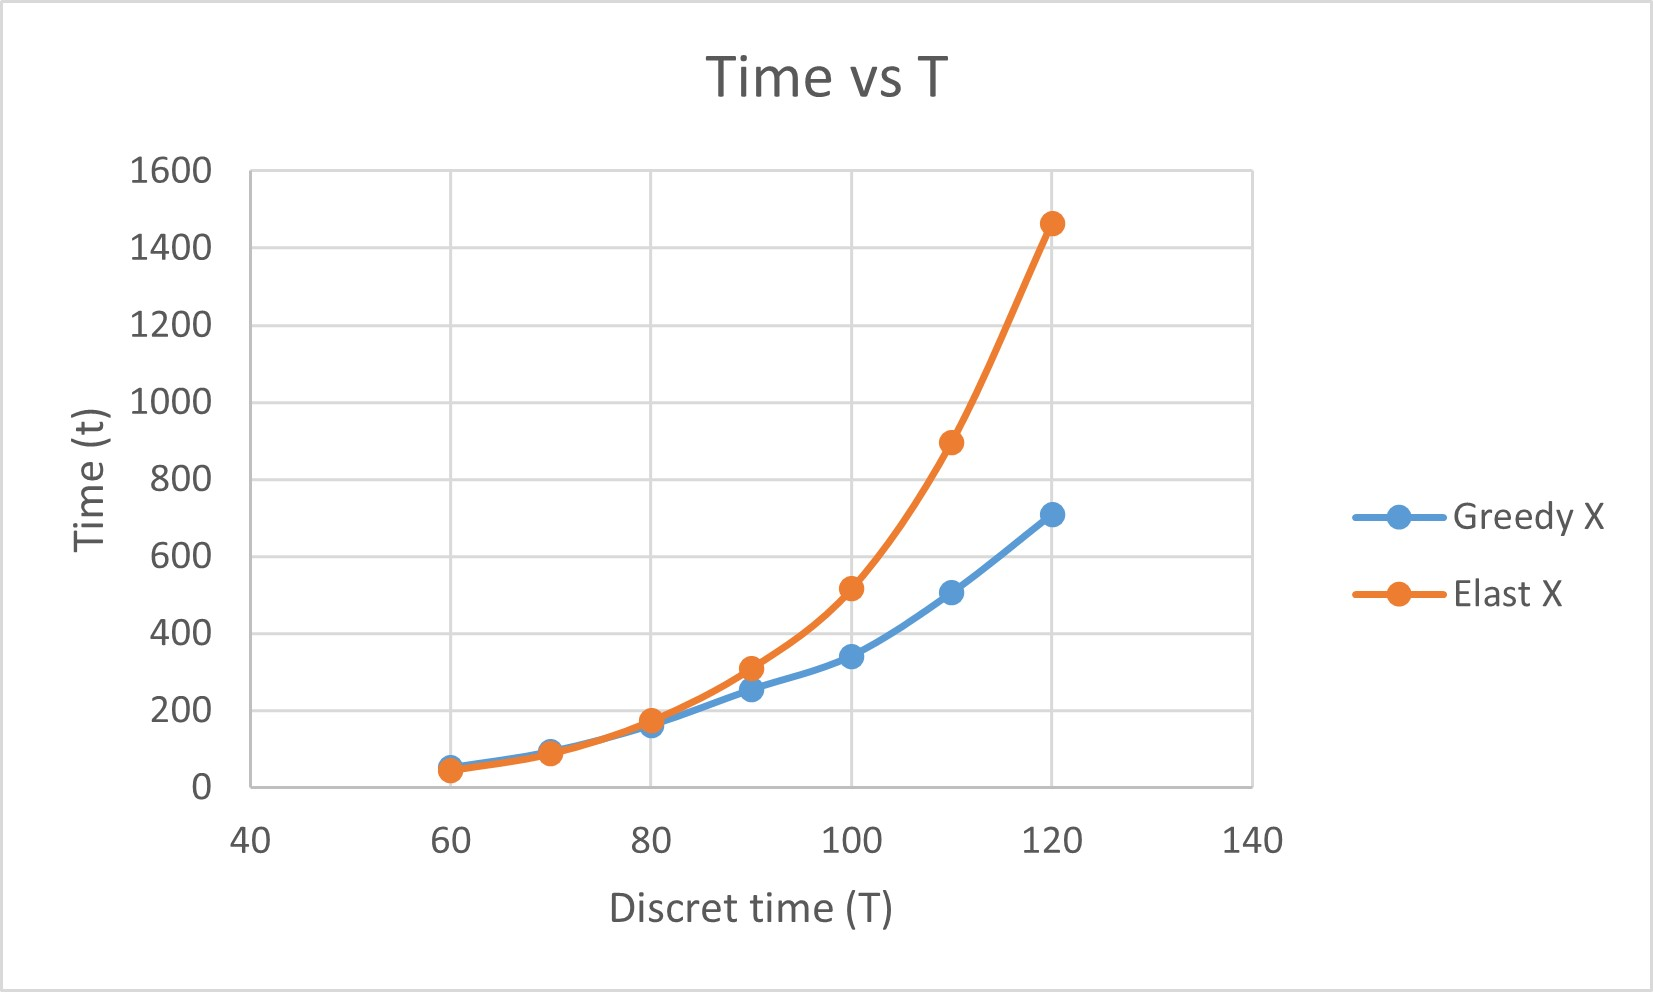
\includegraphics[width=0.75\textwidth]{BothStudyLong.jpg}
\caption{Both study} 
\label{BothStudy}
\end{figure}

\begin{figure}
\centering
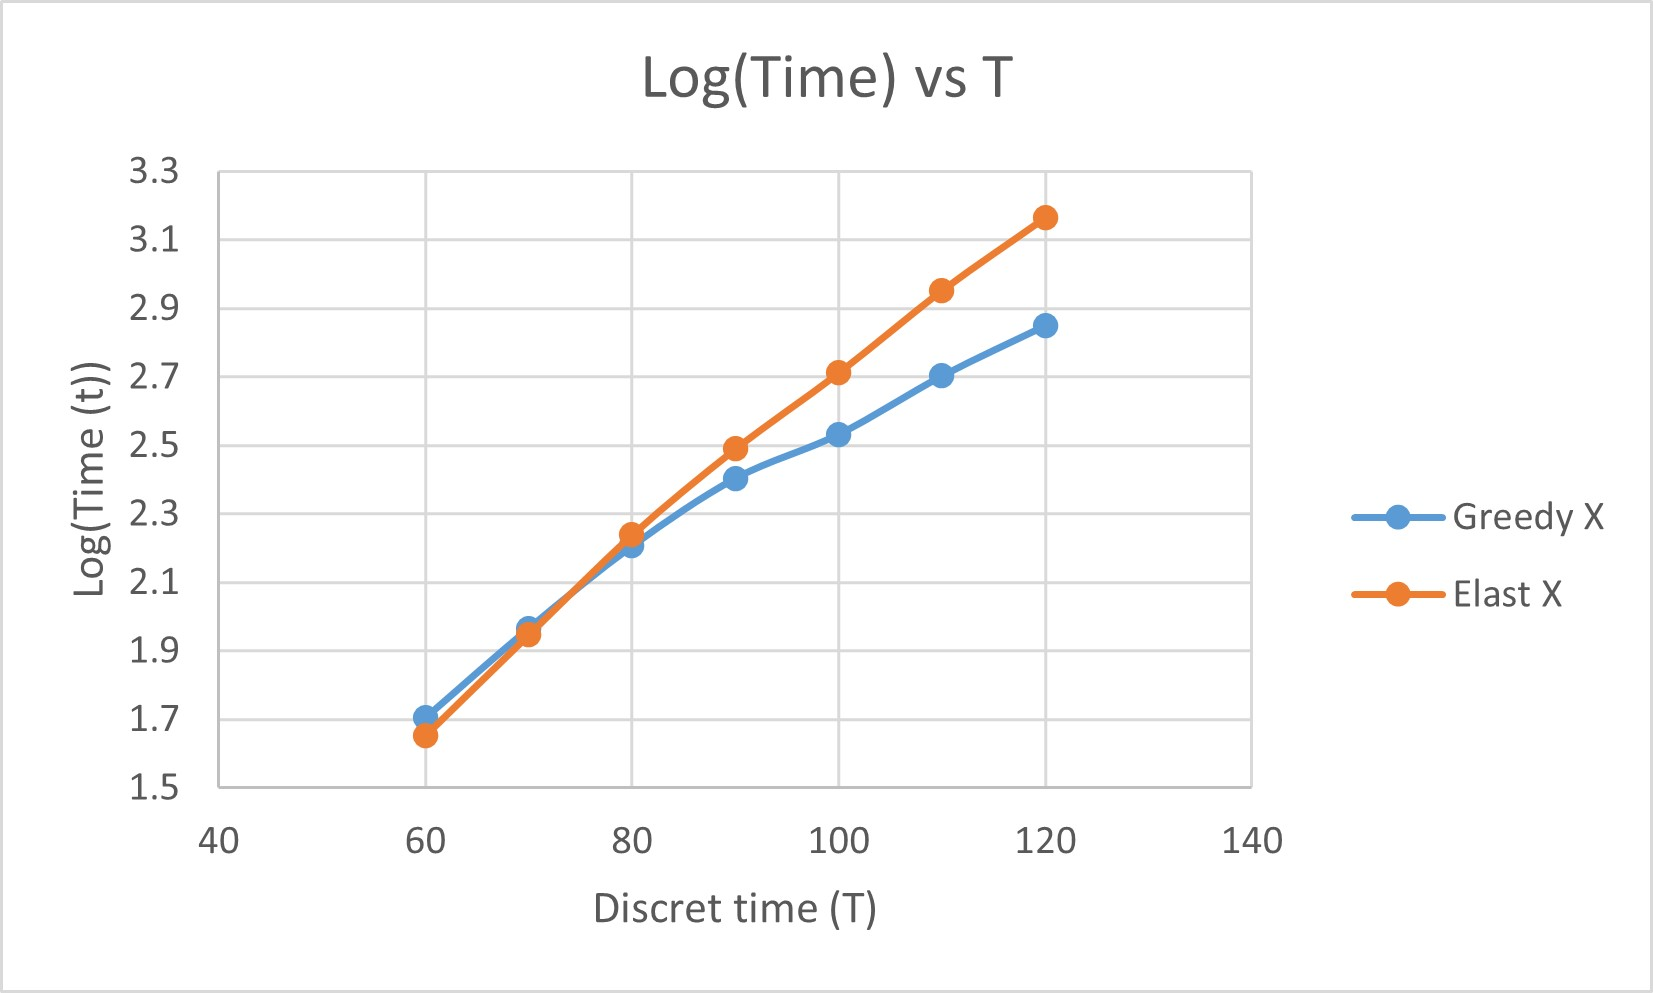
\includegraphics[width=0.75\textwidth]{BothStudyLogLong.jpg}
\caption{Both study (Log scale)} 
\label{BothStudyLog}
\end{figure}

\subsection{A comparative study between the classical and the tensor-based Newmark's methods}

The objective of this section is to show the numerical results obtained for a specific example of the case without damping and another example with damping. These results will be compared with those obtained for the same configuration using an iterative Newmark method. The results are analyzed from three points of view, displacement, velocity and acceleration. For each of them, both the graphs are obtained along the domain for each time instant, as well as the errors between the GROUA and the Newmark method mentioned above.

\subsubsection{A comparative for an elastodynamic model without damping}

The problem treated in the example is a typical case of a beam without taking into account the damping, which is subjected to free vibration, so that no force is exerted on it. The characteristics of the beam and the conditions imposed on it are as follows:

\begin{table}[htb]
\centering
\caption{Beam properties}
\label{tabla:propiedades}
\begin{tabular}{|l|l|}
\hline
\multicolumn{2}{|c|}{Properties} \\ \hline
$m$ & $0.25$ $kg$ \\
$c$ & $0$ $N s/m$\\
$k$ & $1$ $N/m$\\
\hline
\end{tabular}
\end{table}


\begin{table}[htb]
\centering
\caption{Simulation conditions}
\label{tabla:condiciones}
\begin{tabular}{|l|l|}
\hline
\multicolumn{2}{|c|}{Conditions} \\ \hline
$u_0$ & $sen(\pi \tau)$ $m$ \\
$\dot{u}_0$ & $0$ $m/s$\\
$F$ & $0$ $N$\\
$f_0$ & $0$ $N$\\
$L$ & $1$ $m$\\
$T$ & $0.4$ $s$\\
$\gamma$ & $1/2$\\
$\beta$ & $1/6$ \\
$C_0$ & $80409.99$ $m$ \\
$N_x$ & $30$  \\
$N_t$ & $20$  \\
\hline
\end{tabular}
\end{table}

As previously mentioned, the stability of the calculation has been studied, obtaining the value of the constant $C_0$ that can be seen in the table \ref{tabla:condiciones}. Using this value, it is verified that the calculation is stable for all displacement obtained.\\

%%Imágenes desplazamiento

\begin{figure}
 \centering
  \subfloat[Displacement]{
   \label{DespVSDiv}
    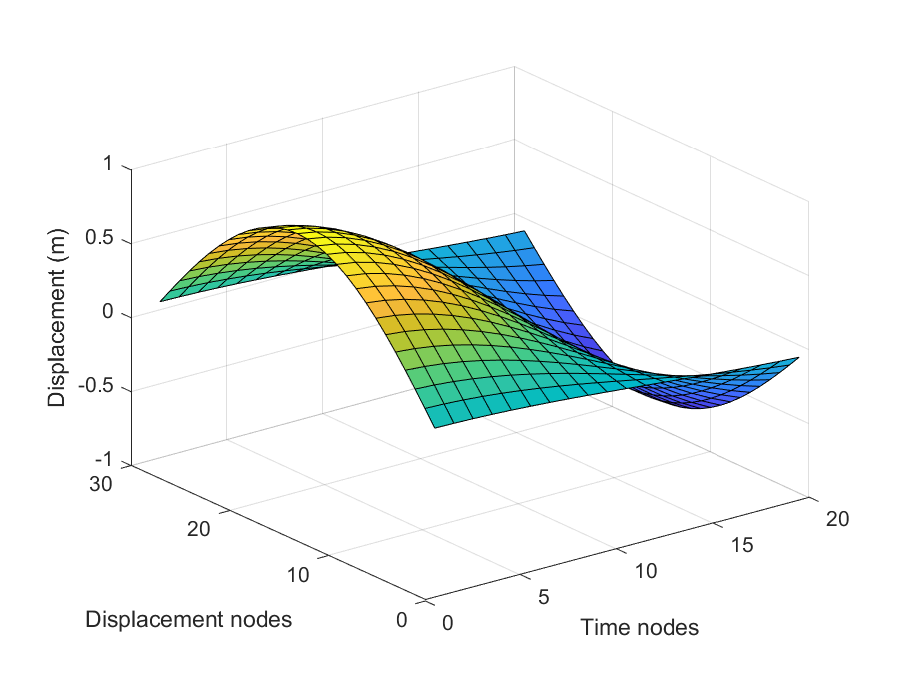
\includegraphics[width=0.5\textwidth]{DispVSDiv_Sup.eps}}
  \subfloat[Displacement error]{
   \label{DespErrVSDiv}
    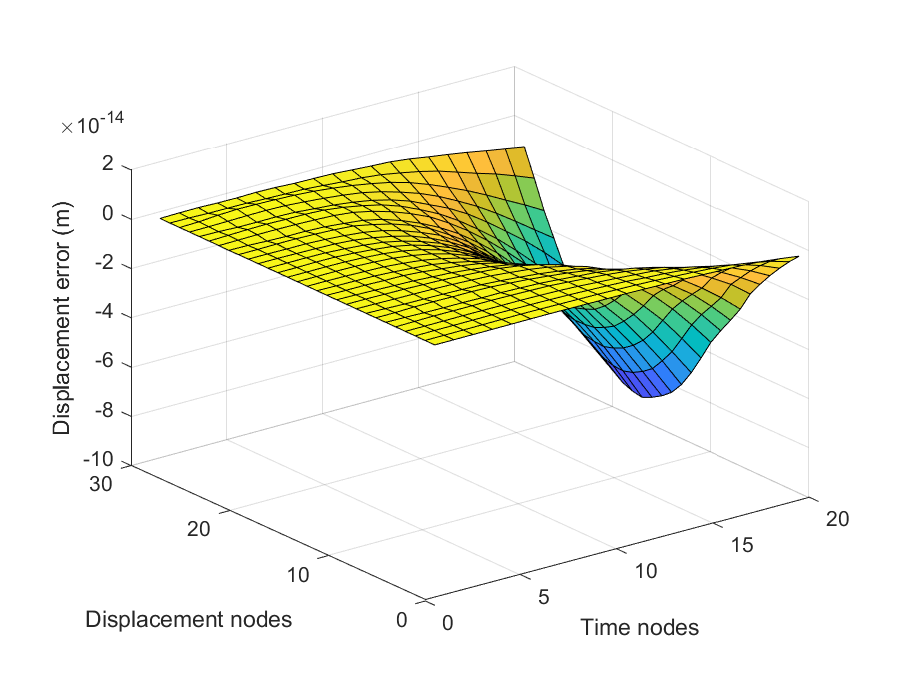
\includegraphics[width=0.5\textwidth]{DispErrVSDiv_Sup.eps}}
  \caption{Displacement and displacement error along the domain without damping}
 \label{DespVSDiv2}
\end{figure}



By imposing as an initial condition a displacement that follows a sinusoidal function, a resulting displacement is obtained like the one in the image \ref{DespVSDiv}, in which the response oscillates between a maximum and a minimum. As for the error obtained, it can be considered negligible as can be seen in the figure \ref{DespErrVSDiv}, since its order is very small compared to the values used in the problem.\\

%%Imágenes velocidad


\begin{figure}
 \centering
  \subfloat[Velocity]{
   \label{VelVSDiv}
    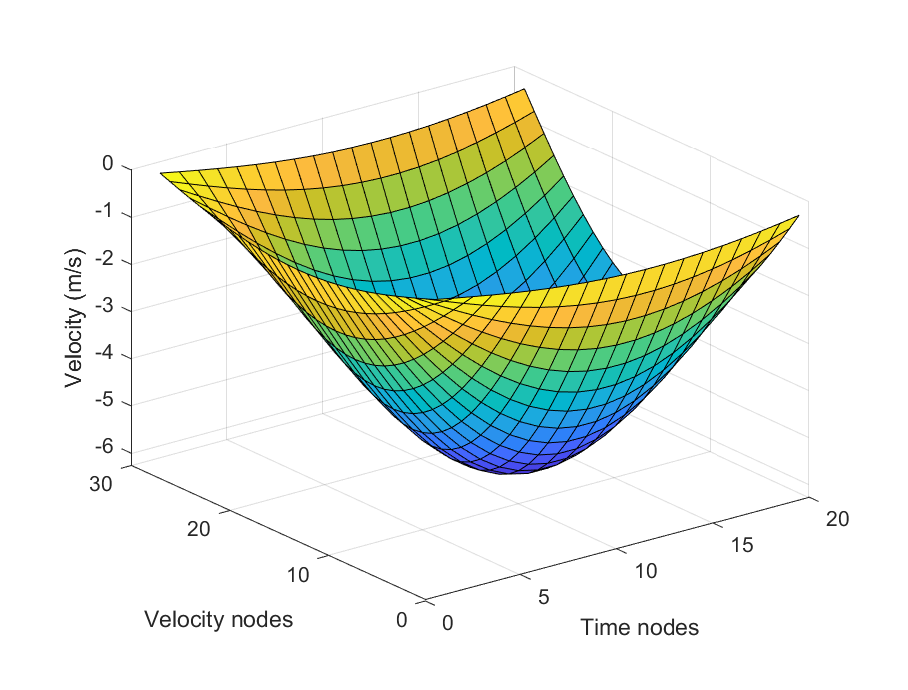
\includegraphics[width=0.5\textwidth]{VelVSDiv_Sup.eps}}
  \subfloat[Velocity error]{
   \label{VelErrVSDiv}
    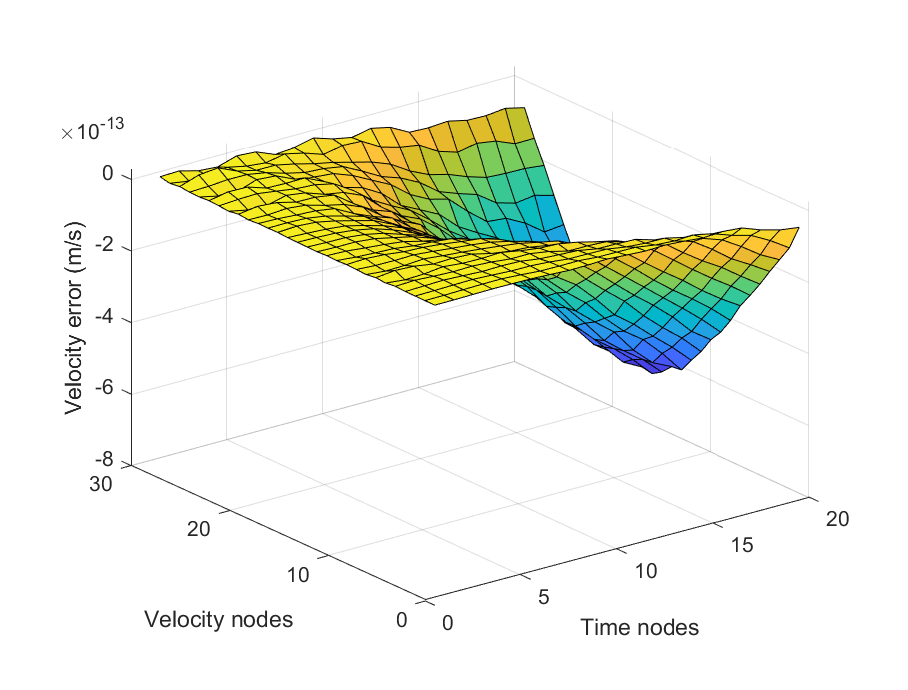
\includegraphics[width=0.5\textwidth]{VelErrVSDiv_Sup.eps}}
 \caption{Velocity and velocity error along the domain without damping}
 \label{VelVSDiv2}
\end{figure}




%%Imágenes aceleracion



\begin{figure}
 \centering
  \subfloat[Acceleration]{
   \label{AccVSDiv}
    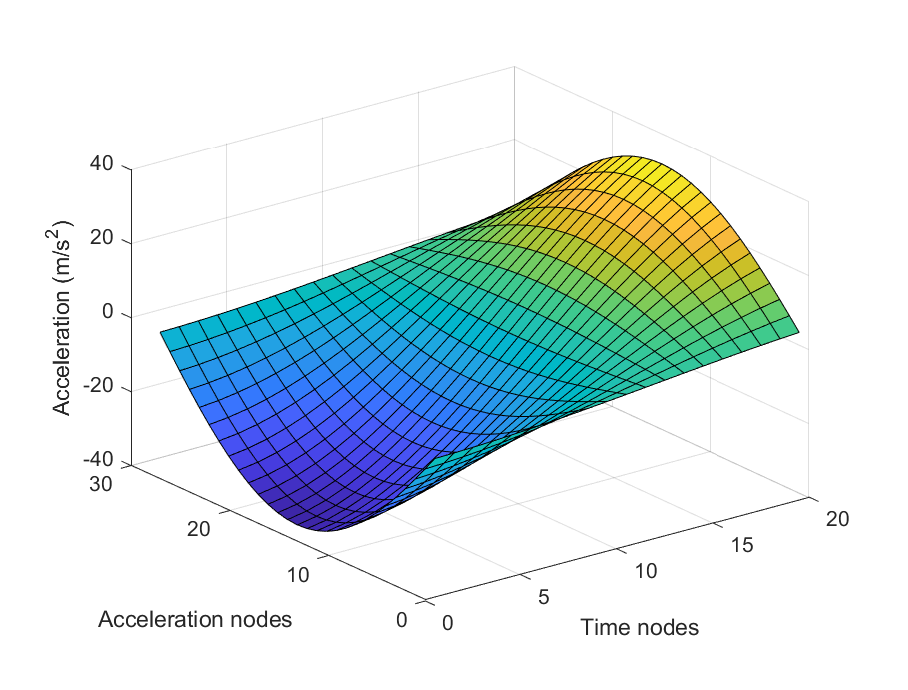
\includegraphics[width=0.5\textwidth]{AccVSDiv_Sup.eps}}
  \subfloat[Acceleration error]{
   \label{AccErrVSDiv}
    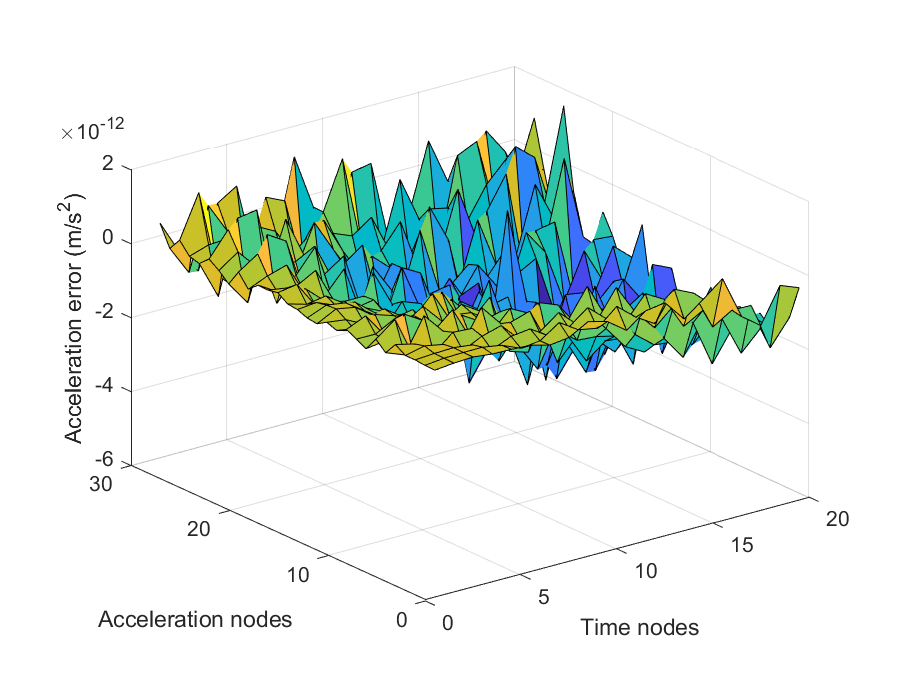
\includegraphics[width=0.5\textwidth]{AccErrVSDiv_Sup.eps}}
 \caption{Acceleration and acceleration error along the domain without damping}
 \label{AccVSDiv2}
\end{figure}



In a similar way to what happens with displacement, the graphs obtained for velocity and acceleration (figures \ref{VelVSDiv} and \ref{AccVSDiv}) are consistent. The error obtained increases by one order of magnitude for velocity and by two for acceleration, as can be seen in the figures \ref{VelErrVSDiv} and \ref{AccErrVSDiv}. Despite this, the error is essentially the same as that obtained for the displacement, since the values that are handled in the velocity and acceleration increase in the same way.\\

Algo muy interesante que se puede observar en las figuras de los errores es que dicho error aumenta con el tiempo. Es lógico pensar que existe un error en el GROUA debido a la propagación que ocasiona este aumento. Pero la realidad es que este error debe ser producido por la propagación del método de Newmark lineal, ya que, como se ha comentado, éste es secuencial en el tiempo. Como se comentará en las conclusiones, el hecho de que el GROUA mejore en gran medida dicho error puede ser una de las fortalezas más importantes en el empleo del GROUA frente a otros métodos.


\newpage

\subsubsection{A comparative for an elastodynamic model with damping}


As in the previous section, the results obtained by GROUA and the iterative Newmark method will be compared, but for a case with relatively simple and two-dimensional damping. The study of a two-dimensional case is already of great interest in itself, since it could simulate a transverse load on something similar to a beam. The analysis of results is the same as the one carried out previously, being the graphs obtained and the procedure followed the same. The example deals with a beam subjected to free vibrations with the following characteristics and conditions:
 
\begin{table}[htb]
\centering
\caption{Beam properties}
\label{tabla:propiedadesD}
\begin{tabular}{|l|l|}
\hline
\multicolumn{2}{|c|}{Properties} \\ \hline
$m$ & $4$ $kg$ \\
$c$ & $1$ $N s/m$\\
$k$ & $1$ $N/m$\\
\hline
\end{tabular}
\end{table}


%%%%%%%%%%%%%%%%%%%%%%%%%%%%%%%%%
\textcolor{Red}{HAY QUE PONER LAS TABLAS BIEN}
%%%%%%%%%%%%%%%%%%%%%%%%%%%%%%%%%

\begin{table}[htb]
\centering
\caption{Beam properties and simulation conditions}
\label{tabla:propiedadesD}
\begin{tabular}{|l|l|}
\hline
\multicolumn{2}{|c|}{Properties} \\ \hline
$m$ & $4$ $kg$ \\
$c$ & $1$ $N s/m$\\
$k$ & $1$ $N/m$\\
\hline
\end{tabular}
\begin{tabular}{|l|l|}
\hline
\multicolumn{2}{|c|}{Conditions} \\ \hline
$u_0$ &  $sen(\pi \tau)$ $m$ \\
$\dot{u}_0$ & $0$ $m/s$\\
$F$ & $0$ $N$\\
$f_0$ & $0$ $N$\\
$L$ & $1$ $m$\\
$T$ & $0.4$ $s$\\
$\gamma$ & $1/2$\\
$\beta$ & $1/6$ \\
$C_0$ & $80409.99$ \\
$N_x$ & $30$ \\
$N_t$ & $20$ \\
\hline
\end{tabular}
\end{table}


\begin{table}[htb]
\centering
\caption{Simulation conditions}
\label{tabla:condicionesD}
\begin{tabular}{|l|l|}
\hline
\multicolumn{2}{|c|}{Conditions} \\ \hline
$u_0$ &  $sen(\pi \tau)$ $m$ \\
$\dot{u}_0$ & $0$ $m/s$\\
$F$ & $0$ $N$\\
$f_0$ & $0$ $N$\\
$L$ & $1$ $m$\\
$T$ & $0.4$ $s$\\
$\gamma$ & $1/2$\\
$\beta$ & $1/6$ \\
$C_0$ & $80409.99$ \\
$N_x$ & $30$ \\
$N_t$ & $20$ \\
\hline
\end{tabular}
\end{table}


As in the case without damping, using the value of $C_0$ it is obtained that the calculation is stable for all the displacements obtained. Due to the initial conditions, the same constant is obtained as in the case without damping.\\


%%Imágenes desplazamiento

By imposing the same initial conditions as before, the effect of damping can be seen clearly, as shown in figure \ref{DespVSDiv}. Compared to the case without damping, a more relaxed transition is observed over time. As main deformation, the complete bending of the beam is observed, but without changes of sign as it happened before. All this is due to the shape of the damping matrix, which is the identity matrix, and the displacement boundary condition 0.\\

As it happened in the cases without damping, the error that exists is very small compared to the displacement values that are handled. Además, en cuanto al error de propagación sucede algo muy parecido al caso sin amortiguamiento.


%Desplazamiento


\begin{figure}
 \centering
  \subfloat[Displacement]{
   \label{DespVSDivAmort}
    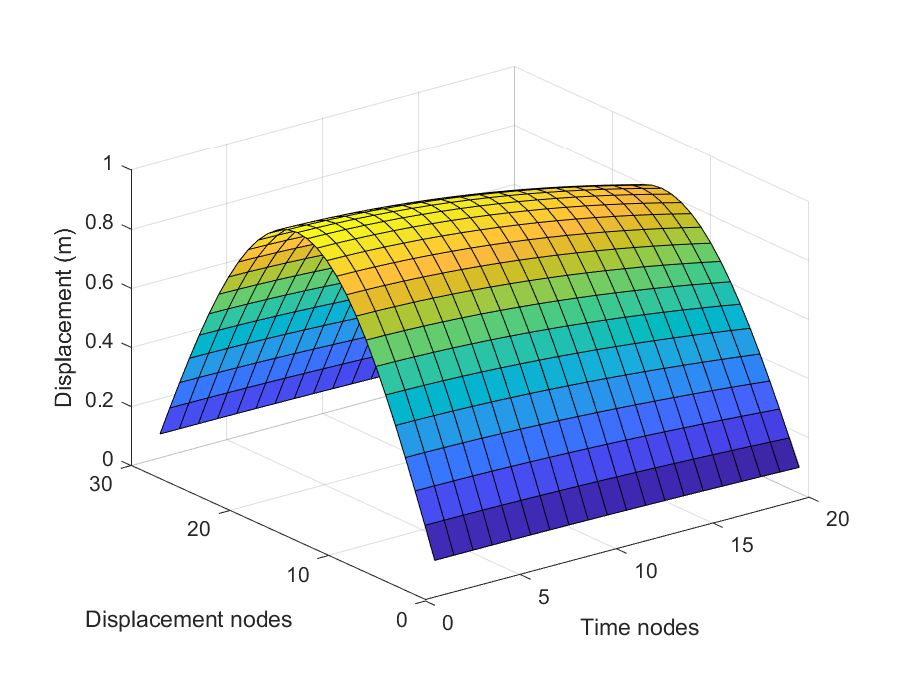
\includegraphics[width=0.5\textwidth]{DispVSDivAmort_Sup.eps}}
  \subfloat[Displacement error]{
   \label{DespErrVSDivAmort}
    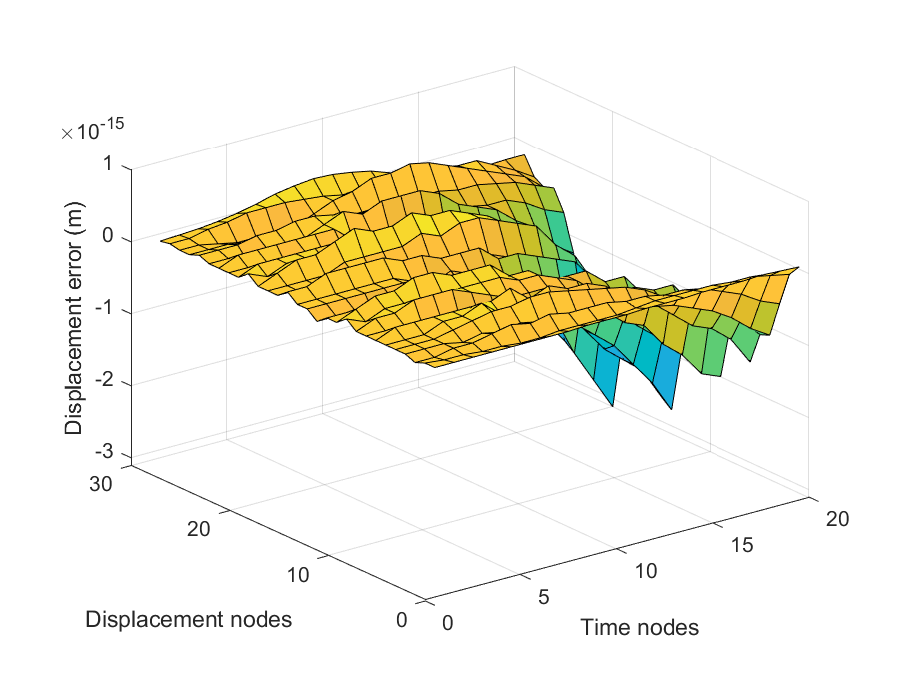
\includegraphics[width=0.5\textwidth]{DispErrVSDivAmort_Sup.eps}}
 \caption{Displacement and displacement error along the domain with damping}
 \label{DespVSDivAmort2}
\end{figure}







%Velocidad


\begin{figure}
 \centering
  \subfloat[Velocity]{
   \label{VelVSDivAmort}
    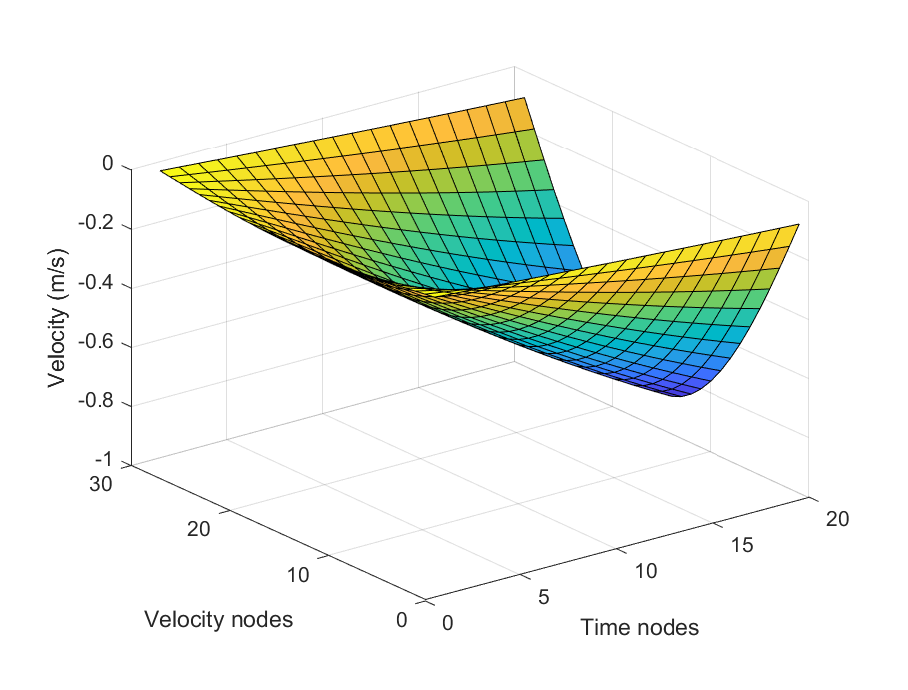
\includegraphics[width=0.5\textwidth]{VelVSDivAmort_Sup.eps}}
  \subfloat[Velocity error]{
   \label{VelErrVSDivAmort}
    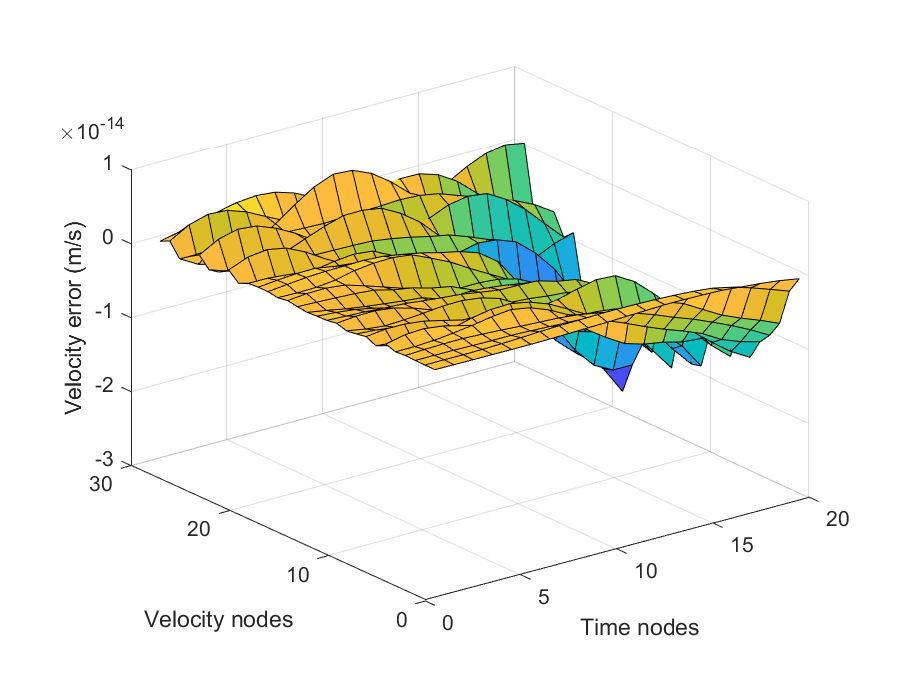
\includegraphics[width=0.5\textwidth]{VelErrVSDivAmort_Sup.eps}}
 \caption{Velocity and velocity error along the domain with damping}
 \label{VelVSDivAmort2}
\end{figure}





%Aceleracion


\begin{figure}
 \centering
  \subfloat[Acceleration]{
   \label{AccVSDivAmort}
    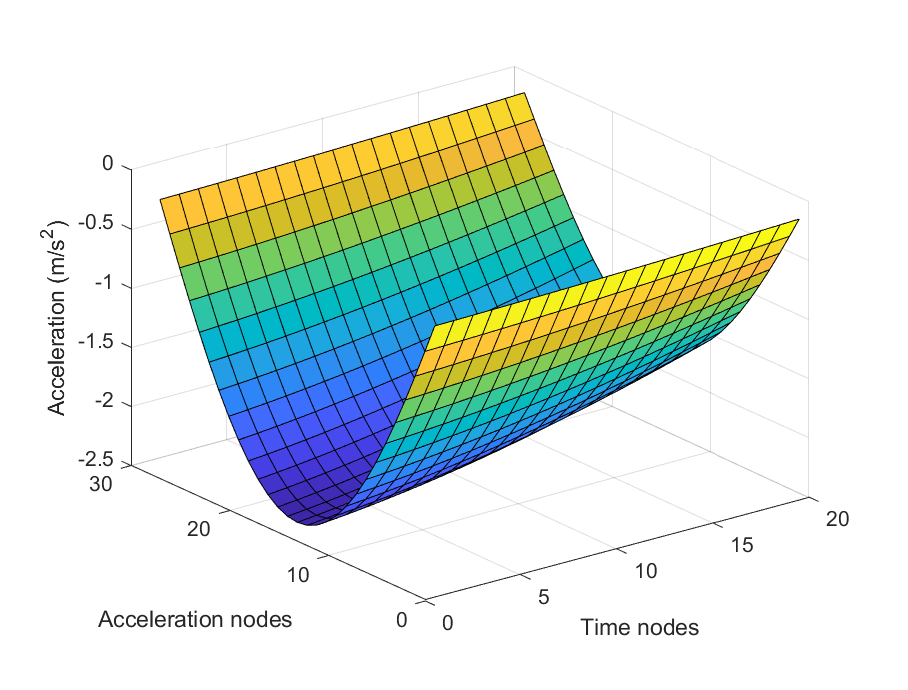
\includegraphics[width=0.5\textwidth]{AccVSDivAmort_Sup.eps}}
  \subfloat[Acceleration error]{
   \label{AccErrVSDivAmort}
    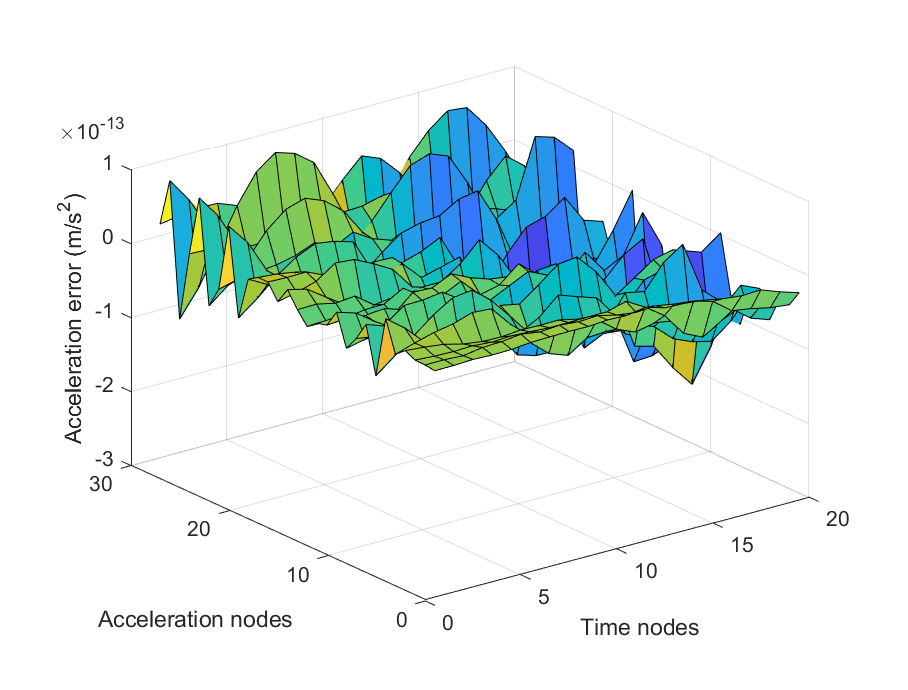
\includegraphics[width=0.5\textwidth]{AccErrVSDivAmort_Sup.eps}}
 \caption{Acceleration and acceleration error along the domain without damping}
 \label{AccVSDivAmort2}
\end{figure}




%%%%%%%%%%%%%%%%%%%%%%%%%%%%%%%%%%%%%%%%
%%%%%% SECCIÓN 6 %%%%%%%%%%%%%%%%%%%%%%%
%%%%%%%%%%%%%%%%%%%%%%%%%%%%%%%%%%%%%%%%

\newpage

\section{Discussion and concluding remarks}

PGD-type methods are a great tool for solving problems with great costs, this has been made clear throughout the entire article. Specifically, the GROUA method used in this article solves problems posed by the elastodynamic equation faster than conventional methods, and also with great precision.\\

In addition to this, it is important to highlight the very basis of GROUA, since with it the entire problem is solved at once, unlike other types of methods, which are sequential. The fact of being sequential gives more fluidity and speed for cases with few elements due to its simplicity at the programming level. But precisely, due to the greater complexity, to a great treatment work on the equations involved, and above all to their tensorization, the GROUA from a certain number of elements turns out to be a much better option.\\

Además,uno de los puntos más a favor del uso de este tipo de métodos es la reducción drástica del error debido a la propagación. La razón es obvia, el hecho de que las ecuaciones se resuelvan prácticamente en una iteración desencadena este fenómeno. Hay que tener en cuenta que, no se puede decir que el cálculo se efectúa en una iteración puesto que, internamente el método realiza varias de ellas. Pero son muy pocas, de hecho en este caso estudiado, son tres.

\textcolor{Red}{Añadir menor error de propagación debido a realizar todo de una, esto se puede ver claramente en las gráficas de errores, donde conforme aumenta el tiempo aumenta el error.}\\

The reality is that using a GROUA to solve today's most complicated engineering problems can be one of the most interesting and fruitful lines of research nowadays.\\


\bibliographystyle{abbrv}
\bibliography{sample}
CHIBA, Fumihiro; KAKO, Takashi. Stability and error analyses by energy estimate for Newmark's method. 1999.
\begin{thebibliography}{99}

\bibitem{JapoStab} CHIBA, Fumihiro; KAKO, Takashi. \textit{Stability and error analyses by energy estimate for Newmark's method}. 1999.

\bibitem{FiniteComputing} LANGTANGEN, Hans Petter; LINGE, Svein. \textit{Finite difference computing with PDEs: a modern software approach}. Springer Nature, 2017.

\bibitem{Ultraweak} HENNING, Julian, et al. \textit{An ultraweak space-time variational formulation for the wave equation: Analysis and efficient numerical solution}. ESAIM: Mathematical Modelling and Numerical Analysis, 2022, vol. 56, no 4, p. 1173-1198.

\bibitem{ConvergenceFalco} AMMAR, Amine; CHINESTA, Francisco; FALCO, Antonio. \textit{On the convergence of a greedy rank-one update algorithm for a class of linear systems}. Archives of Computational Methods in Engineering, 2010, vol. 17, no 4, p. 473-486.









\end{thebibliography}














\end{document}